\documentclass[conference]{IEEEtran}
\IEEEoverridecommandlockouts

\usepackage[utf8]{inputenc}
\usepackage[T5]{fontenc}
\usepackage[english]{babel}

\usepackage{cite}
\usepackage{amsmath,amssymb,amsfonts}
\usepackage{algorithmic}
\usepackage{graphicx}
\usepackage{textcomp}
\usepackage{xcolor}
\usepackage{subcaption}
\usepackage{float}
\usepackage{multirow}
\usepackage[numbers]{natbib}

\def\BibTeX{{\rm B\kern-.05em{\sc i\kern-.025em b}\kern-.08em
    T\kern-.1667em\lower.7ex\hbox{E}\kern-.125emX}}

\renewcommand{\topfraction}{0.95}
\renewcommand{\bottomfraction}{0.95}
\renewcommand{\dbltopfraction}{0.95}
\renewcommand{\textfraction}{0.05}
\renewcommand{\floatpagefraction}{0.95}
\renewcommand{\dblfloatpagefraction}{0.95}

\begin{document}

\title{A Multi-Stage Violence Detection Framework for CCTV Surveillance Using Swin Transformer and Temporal Transformer\\
\thanks{}
}

\author{
    \textbf{1. Hà Như Thái}, \textbf{2. Phạm Tiến Đức}, \textbf{3. Nguyễn Minh Đức}, \textbf{4. Lê Hữu Chính}\\
    \vspace{0.2cm}
    \textit{Posts and Telecommunications Institute of Technology}\\
    Hanoi, Vietnam\\
    \vspace{0.2cm}
    \small
    nhuthai1510@gmail.com, ducpt@ptit.edu.vn, \\
    duc.bc2005@gmail.com, chinh.lh54@gmail.com
}

\maketitle

\begin{abstract}
Most multi-stage violence detection systems for CCTV streams still rely on CNN–LSTM backbones. These pipelines work reasonably well on curated benchmarks, but in our deployment tests they tend to break down when scenes get crowded, when fights are short or partially occluded, and when normal motion (running, hugging, sports) looks visually similar to a real altercation. The failure mode is usually the same: too many false alarms, plus an LSTM that loses track of context once the clip exceeds a few dozen frames.

This paper describes a two-stage framework that we built to address those issues directly. The first stage is a lightweight kinematic filter: we group tracked persons by an adaptive proximity rule, compute seven hand-crafted motion features over a short sliding window, and use an SVM to drop most of the non-violent traffic before any deep model is invoked. The second stage handles the harder cases. We crop the candidate region of interest, feed the 16-frame clip into a Swin Transformer for per-frame spatial encoding, and aggregate the resulting tokens with a small Temporal Transformer instead of a recurrent layer. The two stages share a single goal: send the deep model only the frames it actually needs to look at.

On a unified benchmark of 5,746 clips drawn from six public sources plus our own PTIT footage, the full pipeline reaches 91.2\% accuracy and 91.4\% F1, while running at roughly 24 FPS on a single RTX 2080 Ti. Compared to the CNN–LSTM and attention-based baselines we re-trained under matched conditions, the gain comes mostly from the kinematic gating, which removes obvious negatives before they reach the Transformer.
\end{abstract}

\begin{IEEEkeywords}
Violence detection, CCTV surveillance, Swin Transformer, Temporal Transformer, Multi-stage framework, Spatiotemporal modeling
\end{IEEEkeywords}

\section{Introduction}
Public-area CCTV networks have grown faster than the human capacity to watch them. Modern installations routinely produce thousands of hours of footage per day, and most violent incidents are still discovered hours after they happen, when an operator finally rewinds the right channel. Even when an alert system is in place, human attention degrades after a few hours of monitoring, which means that real fights often go unnoticed while harmless events trigger alarms. Reducing both kinds of error is the practical motivation for automated violence detection.

The dominant family of automated approaches combines a CNN feature extractor with an LSTM (or BiLSTM) for temporal modeling. These pipelines are well studied and easy to train, but they have two recurring weaknesses in real footage. First, occlusion in crowded scenes corrupts the spatial features that the LSTM consumes, and the recurrent state then propagates that corruption forward. Second, fights and non-fights frequently share gross motion statistics: hugging, dancing, sports, and aggressive gesturing all produce high optical-flow energy, and a CNN--LSTM trained on full frames has a hard time separating them without picking up false correlations from the background.

We started this work after observing exactly that pattern on the PTIT campus dataset we collected: a CNN--BiLSTM baseline scored well on RWF-2000 but produced an unworkable false-alarm rate when we deployed it on real classroom and corridor footage. The fix that worked for us was to stop treating violence detection as a single end-to-end problem and split it in two. A cheap kinematic filter throws out the easy negatives (people standing still, walking past, waving), and only the surviving clips are sent to a heavier model. This paper describes how we built each half of that pipeline.

The first stage groups detected persons by an adaptive proximity rule, computes a 7-dimensional motion descriptor over a 10-frame sliding window, and runs an SVM with an RBF kernel as a gatekeeper. The second stage takes the surviving 16-frame ROI clip, encodes each frame with a Swin Transformer~\cite{9710580}, and aggregates the resulting tokens with a small Temporal Transformer. We use a Transformer rather than an LSTM at the temporal layer because the violent events we care about typically span 10--20 frames, and self-attention lets the classifier pick up the approach-contact-recoil pattern even when one or two frames are noisy.

The remainder of the paper is organized as follows. Section~II surveys prior work on violence detection and the spatial--temporal architectures we build on. Section~III walks through the two stages in detail. Section~IV reports the experiments, ablation, sensitivity sweeps, and a comparison with five re-trained baselines. Section~V closes with the limitations we know about and the directions we plan to pursue next.


\section{Related Work}

\label{sec:related_work}

Early work on violence detection in surveillance video used hand-crafted motion and appearance descriptors to flag aggressive behavior~\cite{gracia_fast_2015, ramzan_review_2019, bermejo_nievas_violence_2011}. Typical pipelines mixed frame-differencing, spatio-temporal interest points, and optical flow histograms, sometimes augmented by motion trajectory analysis to catch implausible movements. These descriptors are cheap to compute, but they are also fragile: noise, illumination shifts, and camera shake all break them, which is why they never worked well outside controlled lab footage.

When CNNs took over feature extraction, violence detection followed the same trend~\cite{ding_violence_2014, he_deep_2015, simonyan_two-stream_2014, 7410867}. The two-stream design from Simonyan and Zisserman~\cite{simonyan_two-stream_2014} showed that fusing appearance with dense optical flow gives a clear bump over spatial-only models. The catch is that CNNs see one frame at a time, so they cannot model the sequential nature of a fight, which usually plays out over many frames.

The natural next step was to bolt a recurrent layer on top. CNN--LSTM and CNN--BiLSTM pipelines~\cite{hochreiter1997lstm, patel_realtime_2021, traore_violence_2024, sudhakaran_learning_2017} did improve over spatial-only baselines~\cite{pathak_streamlining_2024}, but they inherited two old problems. The CNN feature is corrupted by occlusion in crowded scenes, and the LSTM then propagates that corruption through its hidden state. On top of that, LSTMs lose grip on long-range temporal dependencies once clips run past a few dozen frames, which is exactly the regime where sustained crowd dynamics produce the most false alarms.

A different line of work goes through pose. By extracting body keypoints with OpenPose~\cite{cao_openpose_2019} and feeding the joint graph through a ST-GCN~\cite{yan_stgcn_2018}, these methods earn some viewpoint and background invariance that pixel-based models cannot match. GNN variants applied at the interaction level~\cite{yun_missiongnn_2024} have posted competitive numbers on curated benchmarks. The drawback is that skeletons themselves are fragile: partial occlusion, low resolution, and large inter-person distances are routine in CCTV footage and routinely produce broken skeleton sequences. GNN approaches also need a person-interaction graph constructed in advance, which makes them sensitive to tracking failures and expensive when the number of people in the scene fluctuates.

A more recent angle is to keep the pixels but split the problem into stages. Multi-stage pipelines~\cite{yun_missiongnn_2024, nguyen_multistage_2021} use a cheap region or motion filter first, then send only the survivors to a deep classifier. Throwing away the background regions early reduces compute and cuts the false alarms caused by bystander movement. Entropy-based filtering is often used as the cheap screening step to reject motion patterns that look superficially like violence but are not.

Transformers have entered this space from a different direction~\cite{vaswani_attention_2023, dosovitskiy_image_2021, bertasius_is_2021, arnab_vivit_2021, pan_violence_2022}. Self-attention links any two positions in a sequence directly, which sidesteps both the sequential bottleneck of RNNs and the locality bias of CNNs. Pan and Fei~\cite{pan_violence_2022} report gains over CNN--LSTM on violence-specific benchmarks. The price is that vanilla video Transformers pay quadratic cost in the number of spatial tokens, which rules out real-time inference on the kind of hardware actually deployed in CCTV systems.

The Swin Transformer~\cite{9710580} addresses the scaling issue by restricting self-attention to local non-overlapping windows and using a shifted-window scheme to share information across them. Compute then grows linearly in the image resolution while the representation stays multi-scale. For violence detection, applying this backbone to cropped interaction regions instead of full frames is doubly useful: token count drops, and the encoder no longer wastes capacity on irrelevant background.

Our work sits at the intersection of these threads. We keep the multi-stage shape from the cascaded pipelines, but we replace the CNN--BiLSTM core with an ROI-based Swin spatial encoder and a light Temporal Transformer over clip-level features. This swap is what lets us hold spatial context for small, occluded interactions while still modeling the long-range temporal pattern that recurrent classifiers struggle with.


\section{Proposed Method}
The hard part of real-time violence detection is not raw model accuracy but separating the rare violent events from the much larger pool of normal activity. Feeding every frame straight into a heavy deep model wastes compute on footage where nothing useful is happening. We therefore split the work into two stages, shown in Fig.~\ref{fig:full_process}. Stage~A is a cheap kinematic screen: it groups tracked persons by an adaptive proximity rule, extracts a 7-dimensional motion descriptor over a short sliding window, and uses an RBF-SVM as a gatekeeper to throw out the obvious negatives. Stage~B picks up the survivors and runs the actual recognition. An ROI-based Swin Transformer encodes the spatial content of each frame, a Temporal Transformer models the clip across time, and an MLP head produces the binary label.

\begin{figure}[!htbp]
    \centering
    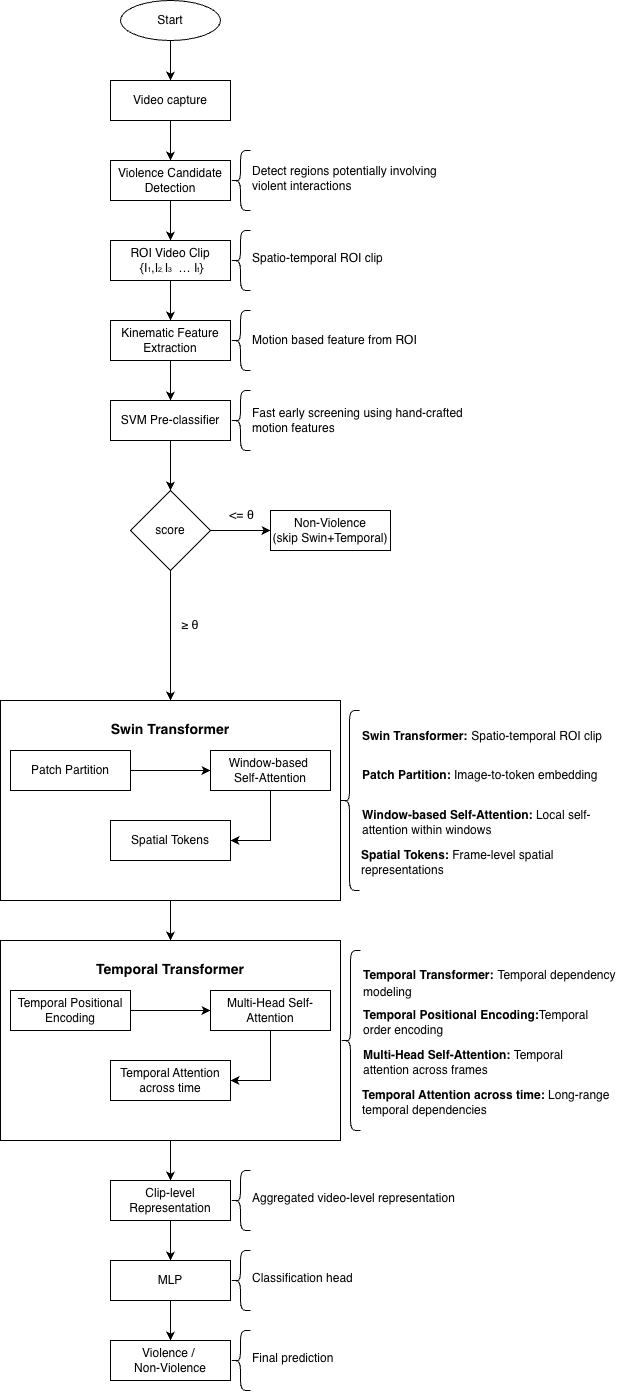
\includegraphics[width=0.75\columnwidth]{image/full_process.png}
    \caption{Overview of the proposed multi-stage violence detection framework. Stage~A performs candidate detection, adaptive grouping, kinematic feature extraction, and SVM-based early screening. Stage~B applies ROI-based Swin Transformer spatial encoding followed by Temporal Transformer modeling for final binary violence prediction.}
    \label{fig:full_process}
\end{figure}

\subsection{High-risk Group Detection and Dynamics-based Preliminary Classification}

Stage~A is the cheap front end of the pipeline. Its job is to spot interactions that might be violent before any deep model is invoked. Fig.~\ref{fig:high_risk_process} shows the flow from raw video to a pass/fail decision. We start by normalizing the input, since incoming clips arrive at very different resolutions and frame rates and physical thresholds need a consistent scale. Persons are then detected and tracked with YOLOv8~\cite{jocher_yolov8_2023} and DeepSORT~\cite{wojke_simple_2017}. The tracked boxes feed an adaptive grouping step that clusters people into interaction groups using a perspective-aware proximity rule. For each group we accumulate a 7-dimensional motion descriptor over a sliding window, capturing kinetic energy, impulse, directional chaos, and optical-flow energy. Two filters then decide whether the window survives: a physics-based threshold for the easy cases, and an RBF-SVM for the borderline ones. The early elimination of normal activity is what keeps the deep stage fast without sacrificing recall on real violent interactions.

\begin{figure}[!htbp]
    \centering
    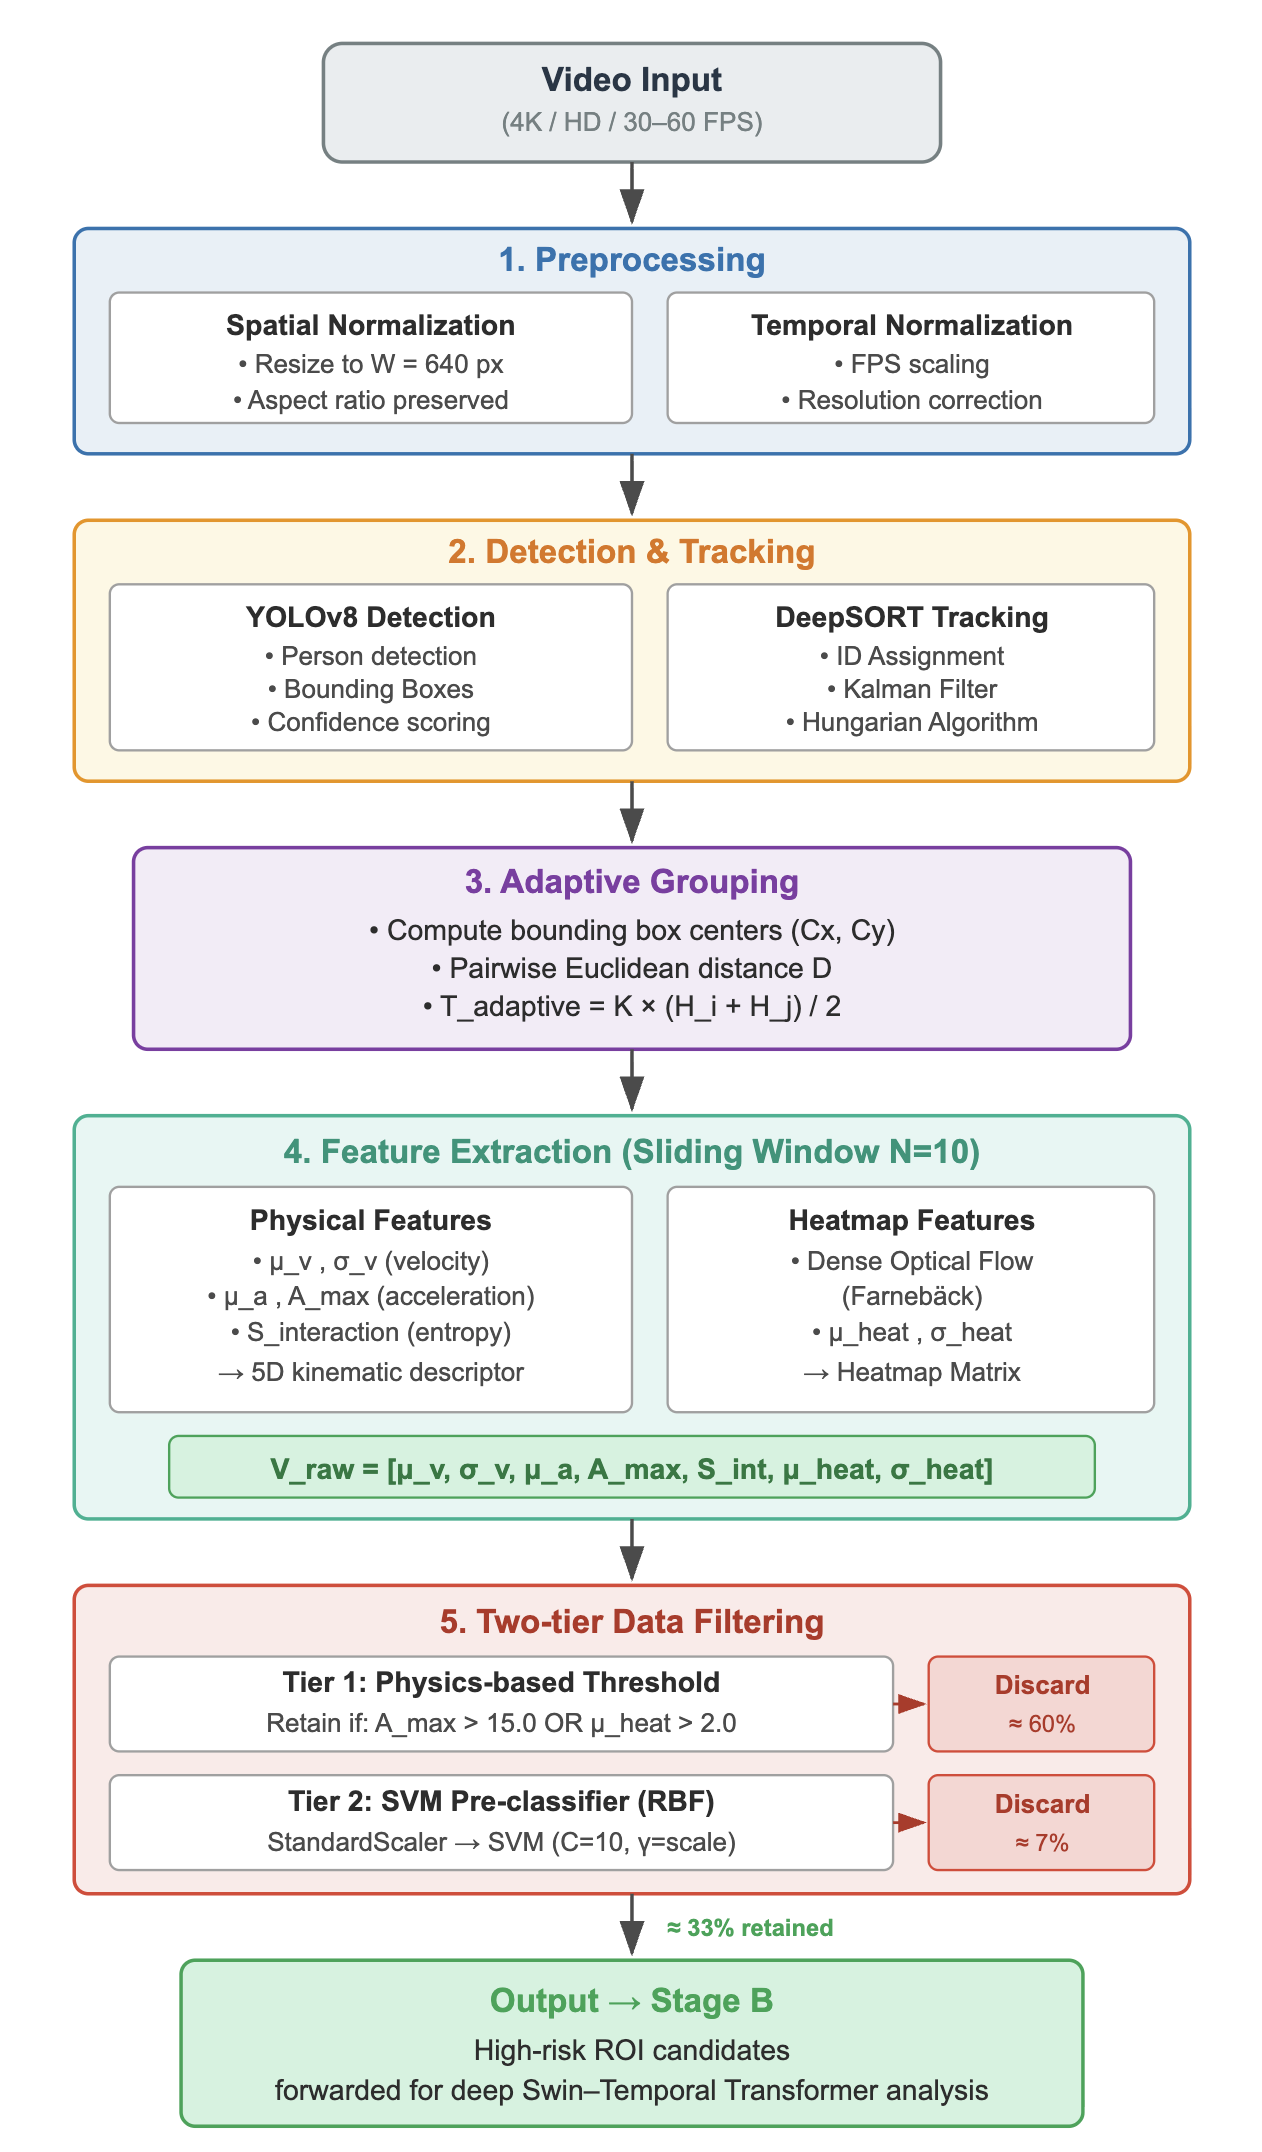
\includegraphics[width=0.85\columnwidth]{image/hig_risk_detect_process_2.png}
    \caption{Detailed pipeline of Stage~A: High-risk Group Detection and Dynamics-based Preliminary Classification. The pipeline processes raw surveillance video through preprocessing, YOLOv8 detection with DeepSORT tracking, adaptive grouping based on scale-aware proximity thresholds, physical and heatmap feature extraction, motion-based data filtering, and SVM classification to produce an early violence risk assessment.}
    \label{fig:high_risk_process}
\end{figure}


\subsubsection{Multi-source Data Normalization and Perspective Adaptation}
Real-world surveillance data is heterogeneous, with wide variation in resolution and frame rate. Applying physical thresholds directly to raw data therefore produces inconsistent results; the same hand gesture produces a much larger pixel displacement in 4K video than in SD. To make the physical calculations comparable across sources, we normalize every input frame to a fixed width of $W_{target} = 640\text{px}$. We picked 640~px because it is the native input resolution of YOLOv8~\cite{jocher_yolov8_2023}, so detection accuracy is preserved without interpolation artifacts, and the optical-flow computation that follows runs faster. Furthermore, velocity and acceleration metrics are scaled by the source video's FPS to ensure temporal invariance.

Following object detection and tracking using YOLOv8~\cite{jocher_yolov8_2023} and DeepSORT~\cite{wojke_simple_2017}, a challenge arises regarding perspective distortion in 2D cameras, which renders interaction distance estimation inaccurate. Instead of using a fixed threshold, we employ an \textit{Adaptive Grouping} mechanism. The interaction threshold $T_{adaptive}$ between two individuals is dynamically calculated based on their own bounding box dimensions:

\begin{equation}
T_{adaptive} = K \times \frac{H_i + H_j}{2}
\label{eq:adaptive_threshold}
\end{equation}

\noindent where $H_i$ and $H_j$ are the heights of the bounding boxes of individuals $i$ and $j$, respectively. Height is selected as the scale proxy because, under perspective projection, a person at greater depth appears shorter in pixel space proportionally to their distance, making $H$ a more reliable and consistent indicator of real-world scale than width. This approach allows the system to self-adjust its sensitivity: the threshold is smaller for distant objects (small boxes) and larger for nearby objects, thereby more accurately reflecting the physical spatial relationship regardless of camera distance.

\begin{figure}[!htbp]
    \centering
    % --- Ảnh (a): Gom nhóm thành công ---
    \begin{subfigure}[b]{\columnwidth}
        \centering
        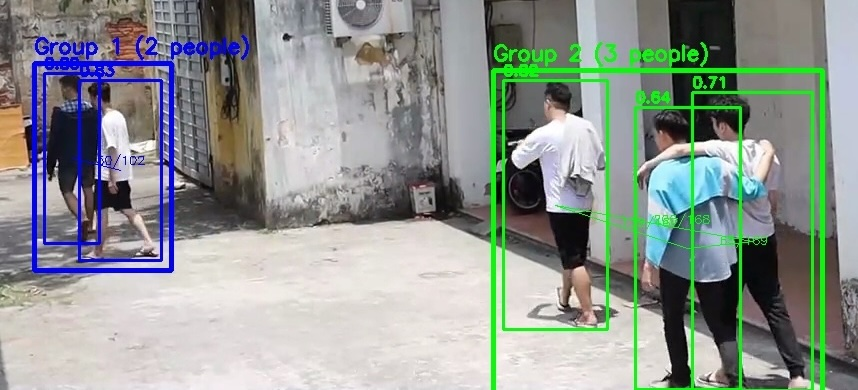
\includegraphics[width=\linewidth]{image/group_people.jpeg} 
        \caption{Successful grouping of interacting individuals}
        \label{fig:grouping_pos}
    \end{subfigure}
    
    \vspace{0.3cm}
    
    % --- Ảnh (b): Phân tách đúng người đi lẻ ---
    \begin{subfigure}[b]{\columnwidth}
        \centering
        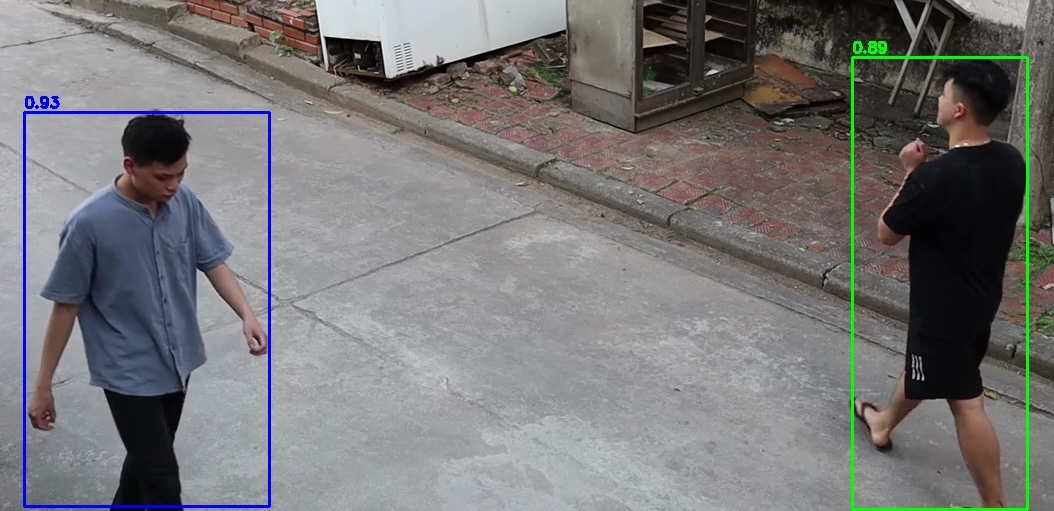
\includegraphics[width=\linewidth]{image/non_group_people.jpeg}
        \caption{Correct separation of independent pedestrians}
        \label{fig:grouping_neg}
    \end{subfigure}
    
    \caption{Validation of the Adaptive Grouping mechanism. (a) Subjects within physical proximity relative to their scale are unified into interaction groups. (b) Pedestrians with spatial gaps exceeding the adaptive threshold are maintained as independent tracks to minimize false alarms.}
    \label{fig:grouping_results}
\end{figure}

The effectiveness of the adaptive grouping mechanism is empirically validated in Fig.~\ref{fig:grouping_results}. In the positive grouping scenario (Fig.~\ref{fig:grouping_pos}), the algorithm successfully identifies two distinct interaction groups from a total of five detected individuals using a scaling factor of $K=1.50$. Group 1, consisting of two subjects positioned further from the camera, exhibits an inter-person distance of $49.75$ pixels against an adaptive threshold of $T_{adaptive}=101.94$ pixels, demonstrating successful grouping despite the relatively small absolute pixel displacement. This behavior exemplifies the scale-invariance property of the adaptive threshold: distant subjects with smaller bounding boxes generate proportionally smaller thresholds, ensuring accurate proximity assessment regardless of depth. Group 2, comprising three individuals in closer proximity to the camera, presents a more complex configuration with inter-pair distances ranging from $64.68$ to $199.84$ pixels and corresponding adaptive thresholds varying between $157.04$ and $169.13$ pixels. Despite the maximum separation of $199.84$ pixels exceeding the average threshold by approximately $18\%$, all three subjects are correctly unified due to the pairwise adaptive nature of the grouping criterion.

Conversely, the negative case illustrated in Fig.~\ref{fig:grouping_neg} demonstrates the algorithm's discriminative capability in preventing false groupings. Two pedestrians walking independently, each forming a singleton group, maintain a spatial separation of $793.77$ pixels. Given their bounding box heights of $H_1=394$ px and $H_2=452$ px, the computed adaptive threshold is $T_{adaptive}=1.50\times(394+452)/2=634.5$ pixels. The actual distance exceeds this threshold by approximately $25\%$, thereby correctly preventing their unification into a single group. This precision is crucial for minimizing computational overhead by excluding irrelevant pedestrian pairs from subsequent motion analysis and reducing false positive detections in crowded surveillance scenarios.


\subsubsection{Micro-physical Feature Extraction}
At each timestamp $t$, the system calculates instantaneous physical metrics for each individual in a group. A critical aspect of our method is the \textit{height normalization} technique. The instantaneous velocity $v_t$ is divided by the object's height ($H_t$), eliminating depth-induced errors and transforming pixel velocity into an index representing the relative energy consumption of the body:

\begin{equation}
v_t = \frac{\sqrt{(x_t - x_{t-1})^2 + (y_t - y_{t-1})^2}}{H_t} \times \text{FPS}
\label{eq:velocity}
\end{equation}

\noindent Instantaneous acceleration ($a_t$) and movement direction angle ($\theta_t$) are also computed to serve as the basis for the subsequent aggregation step.

\subsubsection{Visual Feature Extraction and Heatmap Representation}

In addition to analyzing bounding box coordinates, we extract visual features to capture subtle movements that the bounding box centroid may overlook, such as the rapid motion of limbs. We employ the Farneback Dense Optical Flow algorithm~\cite{farneback_2003} on two consecutive grayscale frames, $I_{t-1}$ and $I_{t}$. The conversion to grayscale is performed to reduce the computational workload and to focus the analysis on light intensity changes rather than chromatic information.

For each pixel $(x, y)$, the algorithm solves the displacement equations to determine the motion vector $V = (u, v)$, where $u$ and $v$ represent the horizontal and vertical displacement components, respectively. Subsequently, a motion energy representation, termed the "Heatmap," is constructed based on the magnitude of these vectors:

\begin{equation}
M(x, y) = \sqrt{u^2 + v^2}
\label{eq:heatmap_magnitude}
\end{equation}

The resulting heatmap $M(x, y)$ is a single-channel matrix where the brightness of each pixel is directly proportional to the movement speed at that specific location. Regions with high-intensity movements, such as punches or kicks, appear as bright, vibrant areas, whereas static objects result in black pixels ($M \approx 0$). This representation provides a localized, intuitive visualization of the motion intensity within the identified Region of Interest (ROI), serving as a crucial visual descriptor for distinguishing between normal and violent interactions. The use of optical flow as a complementary motion representation follows established practices in action recognition~\cite{simonyan_two-stream_2014} and violence detection~\cite{gracia_fast_2015}.
\begin{figure}[!htbp]
    \centering
    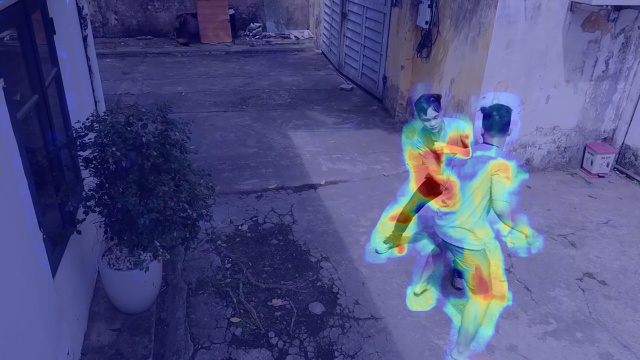
\includegraphics[width=\columnwidth]{image/heatmap_violence.jpeg}
    \caption{Illustration of the combined physical and visual feature analysis for a detected violent interaction. The heatmap visualization demonstrates the spatial distribution of motion energy, with intense activity (red regions) concentrated in the altercation area while static background elements (walls, trees) are suppressed. The 7-dimensional feature vector $V_{raw}$ shows the typical signatures of violent behavior: maximum acceleration $A_{max}=74.42$ (about $5\times$ the safe threshold of $15.0$), interaction entropy $S_{interaction}=103.03^\circ$ indicating directional chaos, and elevated heatmap variance $\sigma_{heat}=2.96$ reflecting localized motion concentration.}
    \label{fig:heatmap_analysis}
\end{figure}

The effectiveness of combining physical and visual feature descriptors is concretely illustrated in Fig.~\ref{fig:heatmap_analysis}. In this frame, the system detects Group 1 consisting of two individuals (ID 2 and ID 3) engaged in physical altercation. From a visual perspective, the heatmap accurately reflects the energy distribution: static background regions (walls, vegetation) are completely suppressed (cold blue tones, $M \approx 0$), while the conflict zone concentrates maximum energy (bright red). This results in a heatmap variance index ($\sigma_{heat}$) of $2.96$, indicating pronounced contrast between subjects and background.

More importantly, analysis of the 7-dimensional feature vector $V_{raw}$ reveals strong alignment with the impulse and chaos hypotheses. Although the group's mean velocity is relatively high ($\mu_v \approx 69.49$), the decisive indicator is the Maximum Acceleration ($A_{max}$) reaching $74.42$ — far exceeding the safety threshold of $15.0$. This value represents the abrupt velocity change (jerk) characteristic of punches or forceful impacts. Simultaneously, the Interaction Entropy ($S_{interaction}$) registers $103.03^\circ$, evidencing that the two subjects are moving in opposing or chaotic directions, distinctly different from the parallel motion of pedestrians walking together. The combination of these indicators triggers a Violence Risk alert, enabling the system to accurately localize the event for subsequent processing.

\subsubsection{Feature Vector Aggregation and Dynamic Analysis}
Violent behavior rarely occurs as a single isolated frame but rather as a sequence of continuous fluctuations. Therefore, we establish a sliding window of size $N=10$ frames. From the raw data collected within this window, we perform statistical aggregation to compress temporal information into a fixed spatial representation. The result is a 7-dimensional feature vector, denoted as $V_{raw}$, defined as follows:

\begin{equation}
V_{raw} = [\mu_v, \sigma_v, \mu_a, A_{max}, S_{interaction}, \mu_{heat}, \sigma_{heat}]
\label{eq:feature_vector}
\end{equation}

\noindent Each component in this vector is designed to capture a specific physical aspect of the behavior:

\begin{itemize}
    \item \textbf{Kinetic energy ($\mu_v, \sigma_v$):} We take the mean and standard deviation of normalized velocity. $\mu_v$ tracks the average energy of the group; a static group has $\mu_v \approx 0$. The mean alone is not enough though, because jogging and fighting can both register a high $\mu_v$. The standard deviation $\sigma_v$ captures the difference: violent motion is jerky (lunges followed by pauses), so $\sigma_v$ comes out much higher than for smooth, harmonic motion at the same speed.

    \item \textbf{Impulse ($\mu_a, A_{max}$):} We put more weight on the maximum acceleration $A_{max}$ within the window than on the mean. Punches and kicks happen very quickly and produce a short acceleration spike that the mean tends to wash out, so $A_{max}$ is the more reliable signal for high-intensity impact. We keep $\mu_a$ as well because it provides a baseline against which $A_{max}$ can be compared.

    \item \textbf{Directional chaos ($S_{interaction}$):} The interaction entropy is the standard deviation of movement angles $\sigma_{\theta}$ across the group. People walking together or fleeing in the same direction produce nearly parallel velocity vectors, so $\sigma_{\theta}$ stays low. A brawl scatters directions: one person lunges forward, another recoils, a third falls. The angle spread shoots up. We use this entropy as our cheap proxy for "is the group moving coherently or not".

    \item \textbf{Visual energy ($\mu_{heat}, \sigma_{heat}$):} Bounding-box motion misses limb-level activity, so we add an optical-flow heatmap on top. $\mu_{heat}$ aggregates the total flow magnitude inside the ROI, picking up small but fast movements (a thrown punch, a swinging arm) that the box centroid does not see. $\sigma_{heat}$ measures how concentrated that motion is in space: a punch creates a localized bright spot against a mostly dark background, which gives a high standard deviation.
\end{itemize}


\subsubsection{Filtering Mechanism and Early Classification}

To optimize real-time performance, we design a two-step filtering process applied to each temporal window sample (each $V_{raw}$ vector aggregated from the most recent 10-frame sliding window of a given interaction group). The first step is a physics-based thresholding filter that immediately discards samples exhibiting low motion intensity. A window sample is retained as a violence candidate only if it satisfies the impulse condition ($A_{max} > 15.0$) or the visual energy condition ($\mu_{heat} > 2.0$). These thresholds are derived from empirical observations that routine daily activities such as walking, standing, or casual gesturing rarely produce a velocity variation exceeding 15\% of body height within a sub-second interval. On our training set, this step alone eliminates approximately 60\%
of all temporal window samples, most of which correspond to stationary or low-motion situations.

The $V_{raw}$ vectors that survive the physics filter are subsequently normalized before classification. The components of $V_{raw}$ span very different scales ($A_{max}$ can reach several hundred, while $\sigma_{heat}$ typically fluctuates between 0 and 5), so we apply zero-mean unit-variance normalization (StandardScaler) independently to each feature dimension. This step is critical for the downstream SVM with an RBF kernel, whose decision boundary depends on Euclidean distances between data points; without normalization, high-magnitude features would dominate the classification outcome.

To train the SVM pre-classifier, we construct a dedicated training set from Stage~A pipeline outputs. Specifically, the complete set of training videos (both violent and non-violent) is processed through YOLOv8~\cite{jocher_yolov8_2023} detection, DeepSORT~\cite{wojke_simple_2017} tracking, adaptive grouping, and micro-physical feature extraction. This process yields 4{,}250 
seven-dimensional $V_{raw}$ samples, each corresponding to a single 10-frame sliding window of a particular interaction group at a specific time instant in the video stream. Labels are inherited from the source video: a sample is labeled positive (\textit{violent}) if the source video is annotated as violent and the group under consideration is involved in the violent interaction during the corresponding time span; all remaining samples are labeled negative (\textit{non-violent}). To verify labeling quality, we manually inspect a random subset of 500 
samples and confirm a labeling accuracy of 96.8\%.
The final SVM dataset comprises 1{,}870 
positive and 2{,}380 
negative samples, reflecting the natural class imbalance in surveillance footage where the majority of temporal windows correspond to normal activity. This dataset is partitioned using a stratified 80/20 split, with 80\% allocated to training and hyperparameter optimization and 20\% reserved for independent evaluation.

The normalized vectors are classified by a Support Vector Machine (SVM) with a Radial Basis Function (RBF) kernel, defined as:
\begin{equation}
K(x_i, x_j) = \exp\bigl(-\gamma \|x_i - x_j\|^2\bigr)
\label{eq:rbf_kernel}
\end{equation}

\noindent We picked SVM-RBF~\cite{cortes_svm_1995} for this gating step over alternatives like a small MLP or a tree ensemble. The feature space here is only 7-dimensional, so we are not in a regime where deep learning has any advantage. The RBF kernel handles the nonlinear separation between violent and non-violent windows well in our experiments. And SVM inference is essentially free at our feature size: a few dot products against the support vectors cost less than 1~ms per window, which is invisible inside a 30~FPS pipeline. The two key hyperparameters, the penalty coefficient $C$ and the kernel parameter $\gamma$, are optimized via grid search combined with 5-fold stratified cross-validation on the training partition. The search space covers $C \in \{0.1, 1, 10, 100\}$ and $\gamma \in \{\texttt{scale}, \texttt{auto}, 0.01, 0.1, 1\}$. The optimal configuration is found at $C = 10$
and $\gamma = \texttt{scale}$, 
achieving a cross-validation accuracy of 74.8\%. 

\begin{table}[!htbp]
\centering
\caption{SVM pre-classifier performance on the held-out validation set}
\label{tab:svm_performance}
\begin{tabular}{lccc}
\hline
\textbf{Class} & \textbf{Prec. (\%)} & \textbf{Rec. (\%)} & \textbf{F1 (\%)} \\
\hline
Non-violent & 78.2 & 61.7 & 68.9 \\
Violent     & 60.5 & 77.3 & 67.9 \\
\hline
\textbf{Weighted Avg} & \textbf{70.1} & \textbf{68.9} & \textbf{68.4} \\
\hline
\end{tabular}
\end{table}

The SVM here is a gatekeeper, not the final classifier. Its operating point is set to favor recall over precision: extra non-violent false positives are tolerable, because Stage~B will throw most of them out anyway, but a missed violent window is gone for good. Anything the SVM rejects is excluded from Stage~B and never recovered. To enforce this policy, the SVM decision threshold is adjusted so that violent recall on the validation set reaches at least 77.3\%,
accepting a precision of 60.5\%
at this stage. The moderate precision is by design: any remaining false positives are subsequently handled by Stage~B (Swin + Temporal Transformer). Table~\ref{tab:svm_performance} summarizes the per-class breakdown. The limited discriminative power of a 7-dimensional handcrafted descriptor is expected; the SVM is not intended to replace a deep recognizer but rather to reduce the candidate pool to a manageable size. Overall, the combination of physics-based thresholding and SVM filtering eliminates approximately 67\%
of all temporal window samples (about 60\% from physics thresholding and an additional 7\% from the SVM), forwarding roughly 33\%
of the candidates to Stage~B for deep analysis. The SVM is therefore mainly a refiner: the physics thresholds do the heavy lifting on load reduction, and the SVM cleans up the borderline cases that would otherwise inflate Stage~B's input. At that point, the system extracts a $T = 16$ consecutive-frame ROI sequence centered on the flagged time instant, where the Swin--Temporal Transformer provides the fine-grained spatiotemporal reasoning that the compact physical features cannot achieve.

To quantify Stage~A's impact at the video level (the metric that matters most for deployment), we analyze whether each violent source video generates at least one forwarded window to Stage~B. On the training partition, Stage~A successfully forwards at least one candidate window for \textbf{96.2\%} of all violent source videos, confirming that fewer than 4\% of violent events are permanently suppressed before reaching the deep recognizer. The remaining 3.8\% are mostly slow-escalation scenarios where neither $A_{max}$ nor $\mu_{heat}$ crosses the physics-based thresholds across the entire 10-frame sliding window. We acknowledge this failure mode in the Limitations section. The gap between the clip-level SVM recall (77.3\%) and this video-level recall (96.2\%) is expected: each violent video contains multiple sliding windows, so missing some individual windows does not preclude the deep recognizer from receiving at least one valid candidate per violent event.

The output of Stage~A is a set of flagged temporal windows, each associated with a specific interaction group and timestamp. For each flagged window, we extract the corresponding group's ROI by computing the union bounding box of all tracked individuals within that group, padded by 15\% to preserve peripheral context. A clip of $T = 16$ consecutive frames is then sampled uniformly from a temporal neighborhood extending slightly beyond the original 10-frame analysis window, capturing both the preceding approach phase and the subsequent aftermath. Each frame is cropped to the ROI region and resized to $224 \times 224$ pixels. This clip constitutes the input to Stage~B. By construction, Stage~B processes only the filtered, high-risk candidates rather than the full video stream, inheriting the computational savings established by Stage~A's early elimination of approximately 67\% of all temporal windows.

\subsection{ROI-based Swin–Temporal Transformer}
Stage~A reduces the candidate pool by rejecting interactions with insufficient kinematic evidence, but it cannot tell genuinely violent events apart from confounding activities that share similar motion signatures, such as abrupt physical contact in sports, animated celebrations, or forceful greetings. These ambiguous cases need a spatial and temporal understanding of body posture, relative movement, and interaction dynamics that handcrafted kinematic descriptors cannot provide. Stage~A operates on optical-flow-derived statistics that capture gross motion intensity. Stage~B instead processes raw RGB frames so that appearance-level cues (facial expressions, body posture, object interactions) are available to the classifier. Concretely, Stage~B applies an ROI-based Swin Transformer~\cite{9710580} for hierarchical spatial encoding of the candidate region, followed by a Temporal Transformer encoder for clip-level violence recognition.

\begin{figure}[!htbp]
    \centering
    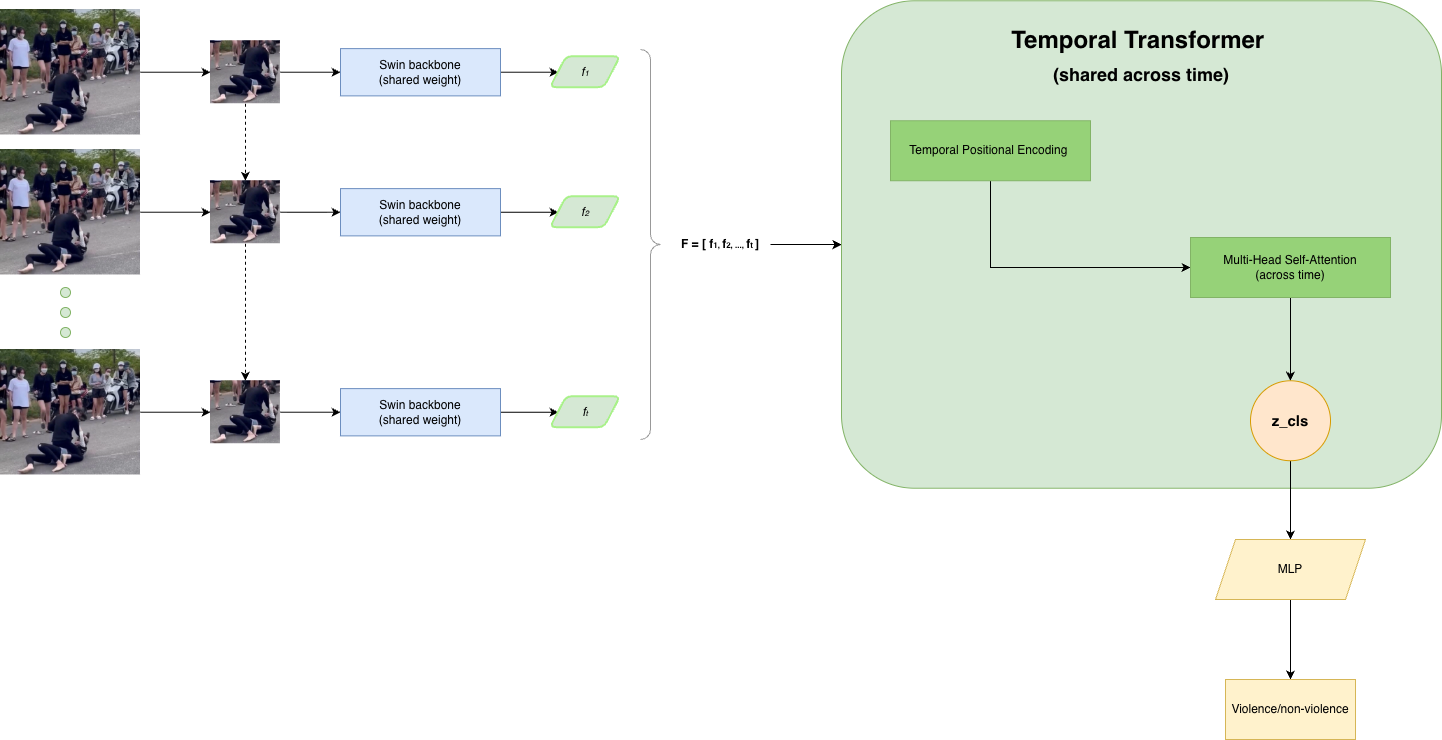
\includegraphics[width=\columnwidth]{image/swin_transformer_process.png}
    \caption{Architecture of the ROI-based Swin--Temporal Transformer module (Stage~B). For each candidate clip, $T$ consecutive ROI frames are independently processed by a shared-weight Swin Transformer backbone to produce frame-level feature descriptors $\{f_1, f_2, \ldots, f_T\}$. The resulting sequence is augmented with temporal positional encoding and passed through a multi-head self-attention encoder that models inter-frame dependencies across the entire clip. The aggregated clip-level representation $z_{\mathrm{cls}}$ is then fed into an MLP classifier to yield the final binary violence prediction.}
    \label{fig:swin_temporal_arch}
\end{figure}


\subsubsection{Swin Transformer for ROI Spatial Feature Extraction}

Violent interactions in surveillance footage are characterized by subtle, spatially compact patterns of physical contact: rapid limb movements, forceful body displacements, and close-range interpersonal dynamics. These cues are easily occluded by neighboring persons or obscured by cluttered backgrounds. Modeling them needs a spatial encoder that can resolve fine-grained local structure while still capturing contextual relationships across the whole interaction region.

The Swin Transformer~\cite{9710580} satisfies both requirements through its hierarchical, window-based self-attention design. Each ROI frame $I_t \in \mathbb{R}^{H \times W \times 3}$ is partitioned into non-overlapping patches, which are projected to embedding vectors via a linear layer. The backbone comprises four stages; at each stage, patch merging progressively halves the spatial resolution while doubling the channel dimension, constructing a multi-scale feature hierarchy. Within each stage, Transformer blocks alternate between window-based multi-head self-attention (W-MSA), which captures intra-window structure at low computational cost, and shifted window-based multi-head self-attention (SW-MSA), which establishes cross-window information exchange. The early stages of this hierarchy retain high-resolution spatial detail, which matters for resolving joint-level interactions such as hand contact or arm extension. Deeper stages then aggregate these local cues into semantically richer representations of body posture and group configuration.

The output of the Swin backbone for each ROI frame $I_t$ is a spatial feature map $F_t$, which is condensed into a single frame-level descriptor via global average pooling (GAP):
\begin{equation}
F_t = f_{\text{swin}}(I_t), \quad z_t = \text{GAP}(F_t) \in \mathbb{R}^d
\end{equation}

\noindent To standardize the descriptor dimension across backbone variants, $z_t$ is passed through a linear projection layer:
\begin{equation}
\tilde{z}_t = Wz_t + b, \quad \tilde{z}_t \in \mathbb{R}^{d_0}
\end{equation}

\noindent where $d_0 = 768$ in our implementation, matching the hidden dimension of the Temporal Transformer encoder.

Restricting Swin encoding to the Stage~A-filtered ROIs rather than the full video frame has two practical effects. The reduction in spatial extent decreases the number of patch tokens processed per forward pass, which keeps throughput high on a continuous CCTV stream. Confining attention computation to the interaction region also suppresses interference from background motion (passersby, vegetation, traffic) that would otherwise dilute the feature representation and raise the false-positive rate downstream.


\subsubsection{Temporal Transformer for Clip-level Violence Modeling}

Violence is a temporally structured event. A typical altercation moves through three phases (approach, physical contact, and recoil), and any one of them, viewed in isolation, can resemble non-violent motion. Frame-level classifiers cannot see this structure at all, and recurrent architectures such as LSTM tend to degrade over longer clips because of cumulative hidden-state error. The Temporal Transformer encoder sidesteps both issues by modeling behavioral dynamics directly in the clip-level feature space through global self-attention over the temporal axis.

For each Stage~A-filtered ROI, a clip of $T$ uniformly sampled frames is constructed:

\begin{equation}
\{I_t\}_{t=1}^{T}
\label{eq:clip_frames}
\end{equation}

\noindent We set $T = 16$, a choice that balances temporal context coverage against per-clip inference latency. To extend the effective observation window without increasing the token count, frames are sampled at a stride of $s$ frames, where $s$ is determined by the source frame rate. In practice we use $s=2$ for 30~FPS sources (covering $\sim$1.07~s per clip) and $s=3$ for 60~FPS sources, ensuring the 16-frame clip spans approximately one second of real time regardless of the source resolution-frame-rate combination.

During training, stochastic temporal augmentations are applied to promote invariance to absolute clip position: random clip start offset, small temporal jitter on the sampling stride, and probabilistic frame dropout. These augmentations are applied independently per clip and do not alter the number of tokens consumed by the Temporal Transformer.

Using the frame-level descriptor $\tilde{z}_t \in \mathbb{R}^{d_0}$ produced by the Swin encoder for each frame, the clip is represented as a matrix:

\begin{equation}
Z = [\tilde{z}_1, \tilde{z}_2, \ldots, \tilde{z}_T] \in \mathbb{R}^{T \times d_0}
\label{eq:clip_matrix}
\end{equation}

\noindent Since self-attention is permutation-invariant, temporal order is injected by adding a learnable positional encoding $P \in \mathbb{R}^{T \times d_0}$ to the token sequence:

\begin{equation}
H^0 = Z + P
\label{eq:positional_encoding}
\end{equation}

\noindent The input $H^0$ is then processed by $L$ successive Transformer encoder layers, each comprising multi-head self-attention (MHSA) over the temporal axis followed by a position-wise feed-forward sublayer and residual connections:

\begin{equation}
H^\ell = \text{TransformerEnc}(H^{\ell-1}), \quad \ell = 1, \ldots, L
\label{eq:transformer_layer}
\end{equation}

\noindent In our configuration, $L = 2$ encoder layers are used, each with $h = 8$ attention heads operating on the full $d_0 = 768$-dimensional space (head dimension $d_k = 96$). A dropout rate of $p = 0.1$ is applied to both the attention weights and the feed-forward activations within each layer to mitigate overfitting on the relatively compact ROI clip dataset.

Self-attention computes pairwise compatibility scores between every pair of temporal positions $(t_i, t_j)$, enabling the encoder to selectively integrate evidence from the approach phase, the moment of contact, and the recoil phase simultaneously. This global receptive field over the clip is the primary architectural advantage over LSTM, which must propagate information sequentially and is prone to gradient attenuation across long time spans.

After $L$ encoder layers, the clip representation $H^L \in \mathbb{R}^{T \times d_0}$ is aggregated via temporal mean pooling:

\begin{equation}
g = \frac{1}{T} \sum_{t=1}^{T} H^L[t] \in \mathbb{R}^{d_0}
\label{eq:temporal_pooling}
\end{equation}

\noindent Mean pooling assigns equal contribution to all frames, which is appropriate given that violent actions may appear at any position within the sampled clip rather than being concentrated at fixed temporal locations.

The pooled vector $g$ is passed through a two-layer MLP with a hidden dimension of $d_0 / 2 = 384$ and ReLU activation, followed by a single linear output unit. The model is optimized end-to-end with binary cross-entropy with logits loss (\texttt{BCEWithLogitsLoss}), which numerically combines the sigmoid activation and binary cross-entropy into a single stable operation:

\begin{equation}
\mathcal{L} = -\bigl[y \log \sigma(\hat{y}) + (1 - y) \log (1 - \sigma(\hat{y}))\bigr]
\label{eq:bce_loss}
\end{equation}

\noindent where $\hat{y}$ is the raw logit output of the MLP and $y \in \{0, 1\}$ is the ground-truth violence label.

Temporal self-attention gives us two concrete practical benefits over frame-level or recurrent classifiers. By jointly attending to all frames, the encoder can pick up approach-contact-recoil transitions whose decisive signal is spread across non-adjacent frames, which LSTM hidden states often fail to preserve intact over 16 time steps. The absence of sequential computation also removes the dependency on error-free tracking continuity: a missed detection on one or two frames does not corrupt the representation of the rest of the clip, because each token is encoded independently before attention is applied.

\subsubsection{Integrating Swin and Temporal Transformer in the Multi-stage Pipeline}

Stage~B only sees ROIs that Stage~A has already forwarded, so it never has to process full frames. Inside the stage, Swin handles spatial encoding for each frame, producing hierarchical descriptors that cover both fine-grained interaction details and broader body-level context. The Temporal Transformer then takes these per-frame descriptors and aggregates them across the clip, ending with a single clip-level vector for the binary classification head.

We deliberately keep spatial and temporal modeling separate. Swin is pretrained on ImageNet~\cite{deng_imagenet_2009} and fine-tuned as a feature extractor, while the Temporal Transformer is trained from scratch on our ROI clip dataset. Splitting the two means each module solves a smaller, better-defined problem, and we have found this easier to optimize than the jointly-trained 3D convolutional alternatives we tried earlier.

The cascade design has two practical benefits that build on each other. Because Stage~B only sees the filtered ROI subset, average GPU utilization per video stays well below what an unconstrained deep recognizer would need on every detected person-group crop. The spatial gating from Stage~A also gives Stage~B a cleaner input distribution: clips that arrive here have already passed a kinematic sanity check, so the easy non-violent samples are gone and the deep classifier can spend its capacity on the truly ambiguous cases.

\begin{figure*}[!t]
\centering
\includegraphics[width=0.9\linewidth]{image/violance.png}\\[0.3em]
{\small (a) True Positives: Violent interactions under varying conditions.}\\[0.8em]
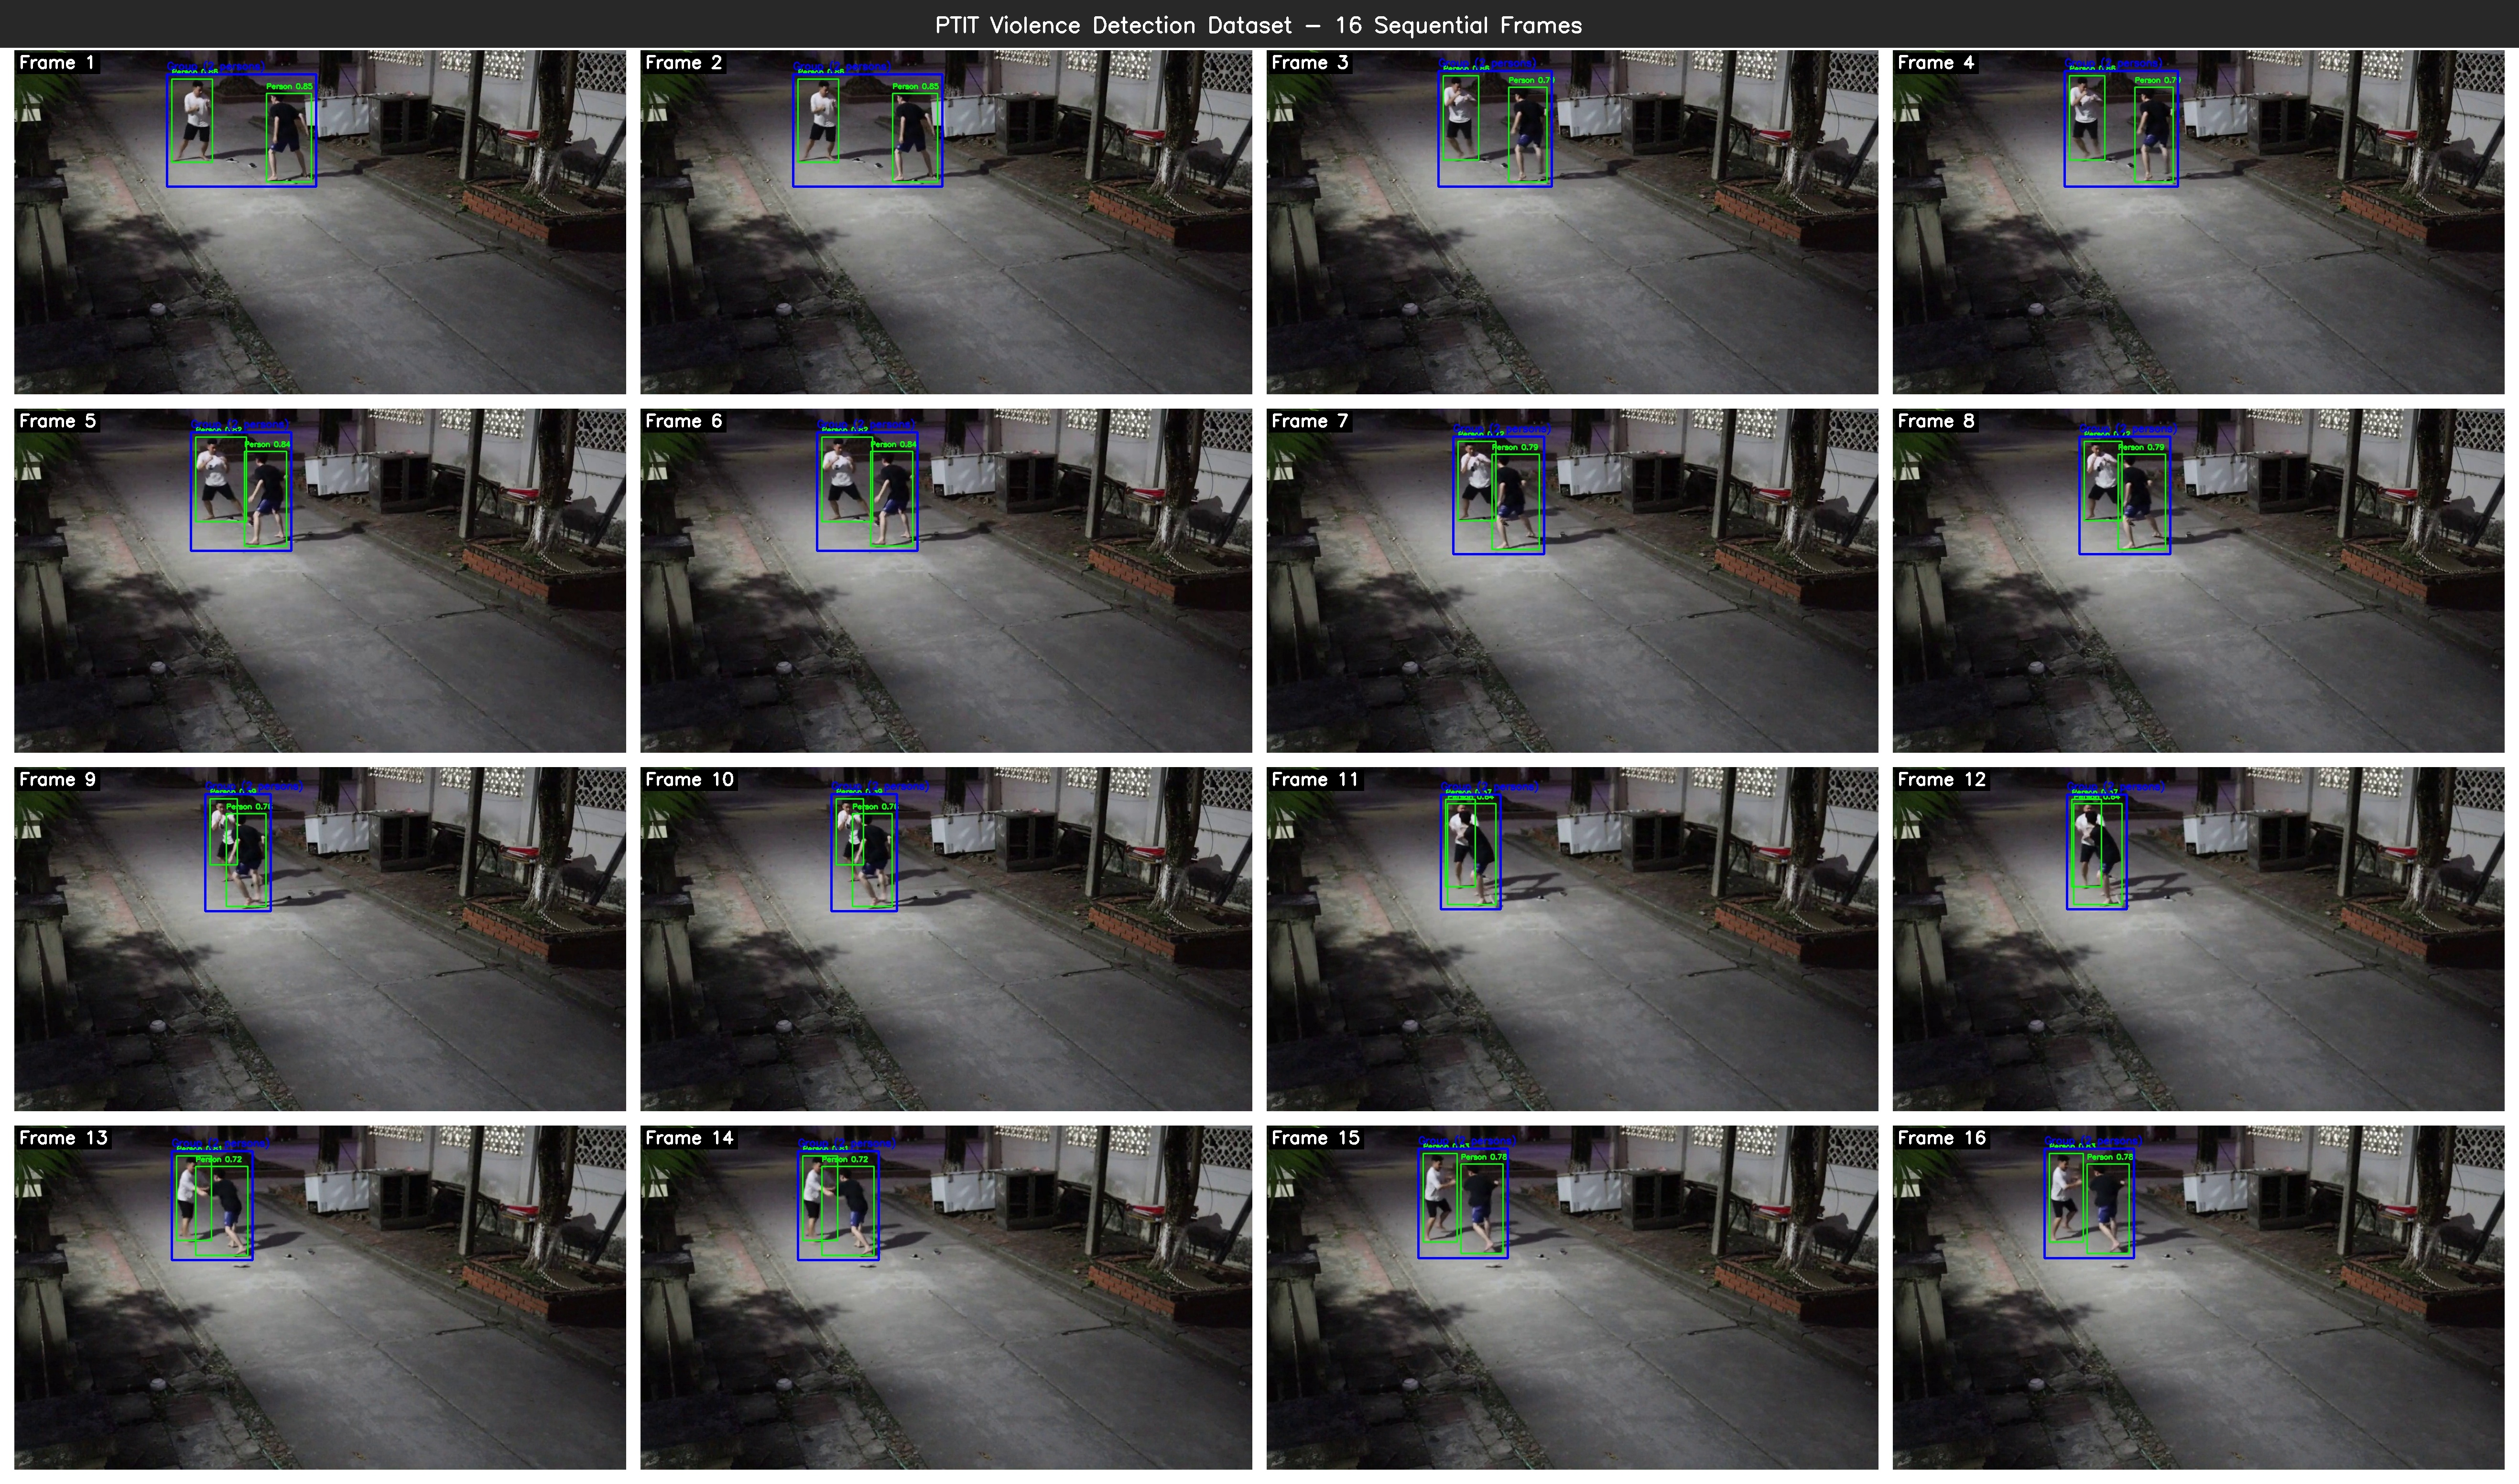
\includegraphics[width=0.9\linewidth]{image/violance_night.jpg}\\[0.3em]
{\small (b) Hard Negatives: Non-violent sequences including hugging, dancing, and fast-moving objects.}
\caption{Sample frames from the Unified Benchmark showcasing both true positive violent events and challenging hard negative scenarios.}
\label{fig:unified_samples}
\end{figure*}

\section{Experimental Results}

\subsection{Datasets and Evaluation Protocols}

We built this framework with real CCTV footage in mind, not the cleaner clips that most public benchmarks ship with. Real cameras deal with awkward angles, mixed lighting, and crowd dynamics that no curated dataset captures on its own, so we pulled raw data from six different sources to keep the test conditions honest.

The combined pool has 5,746 clips, split evenly between violent and non-violent classes. We did an 80/20 stratified split at the clip level and trained on 4,597 of them. The held-out 20\% from each source were merged into a single test set we refer to as the Unified Violence Surveillance Benchmark, which contains 1,149 clips.

\begin{table}[!htbp]
\centering
\caption{Experimental Dataset Distribution}
\label{tab:exp_dataset}
\footnotesize
\begin{tabular}{lcccc}
\hline
\textbf{No.} & \textbf{Dataset} & \textbf{Test} & \textbf{Viol.} & \textbf{Non-Viol.} \\
\hline
1 & RWF-2000~\cite{cheng_rwf-2000_2020} & 2000 & 1000 & 1000 \\
2 & Real Life Violence Situations~\cite{soliman_violence_2019} & 2000 & 1000 & 1000 \\
3 & Hockey Fight~\cite{nievas2011violence} & 1000 & 500 & 500 \\
4 & Auto Violence Detection~\cite{bianculli_dataset_2020} & 350 & 175 & 175 \\
5 & Movies Violence / Non-Violence~\cite{bermejo_nievas_violence_2011} & 246 & 123 & 123 \\
6 & PTIT Dataset (ours) & 150 & 75 & 75 \\
\hline
\textbf{Total} &  & \textbf{5746} & \textbf{2873} & \textbf{2873} \\
\hline
\end{tabular}
\end{table}



Table~\ref{tab:exp_dataset} details the source composition. Table~\ref{tab:test_dataset_description} visualizes the core metadata distributions. The unified benchmark contains resolutions from standard 640$\times$480 to 1280$\times$720 HD. Clip lengths heavily concentrate between 2:37 and 4:00. This structural diversity forces models to handle extreme hardware variations.

\begin{table}[!htbp]
\centering
\caption{Sample Metadata from the Dataset}
\label{tab:test_dataset_description}
\resizebox{\linewidth}{!}{%
\begin{tabular}{|c|c|c|l|c|}
\hline
\textbf{Video Name} & \textbf{Resolution} & \textbf{Total Time} & \textbf{Description} & \textbf{Violence} \\
\hline
VID01 & 1280x720 & 03:02 & Daytime interaction & Violent \\
\hline
VID02 & 1280x720 & 02:45 & Daytime interaction & Violent \\
\hline
VID03 & 1280x720 & 03:21 & Night interaction & Non-Violent \\
\hline
VID04 & 1280x720 & 02:58 & Night interaction & Violent \\
\hline
VID05 & 1024x576 & 03:51 & Close interaction & Non-Violent \\
\hline
VID06 & 1024x576 & 04:00 & Close interaction & Non-Violent \\
\hline
VID07 & 960x540 & 03:25 & Far interaction & Violent \\
\hline
VID08 & 960x540 & 03:41 & Far interaction & Non-Violent \\
\hline
VID09 & 960x540 & 03:56 & Crowded interaction & Violent \\
\hline
VID10 & 854x480 & 02:50 & Crowded interaction & Violent \\
\hline
VID11 & 854x480 & 02:37 & Multiple people interaction & Non-Violent \\
\hline
VID12 & 854x480 & 03:44 & Multiple people interaction & Violent \\
\hline
VID13 & 640x480 & 03:18 & Indoor interaction & Non-Violent \\
\hline
VID14 & 640x480 & 02:59 & Indoor interaction & Non-Violent \\
\hline
VID15 & 1280x720 & 03:35 & Daytime interaction & Violent \\
\hline
VID16 & 960x540 & 03:12 & Far interaction & Non-Violent \\
\hline
VID17 & 854x480 & 02:54 & Night interaction & Violent \\
\hline
VID18 & 1024x576 & 03:27 & Crowded interaction & Non-Violent \\
\hline
\end{tabular}%
}
\end{table}

Figure~\ref{fig:unified_samples} displays raw frames extracted from the test partition. Environmental conditions shift drastically. The top row depicts actual violence, including large-scale brawls occupying the entire field of view alongside localized interactions occurring at greater distances from the camera. The bottom row demonstrates the hard negatives, including hugging, dancing, incidental collisions, and fast-moving objects. These specific samples are selected to directly evaluate the false positive rate of the pipeline.

\subsection{Implementation Details}
We ran every experiment on a single workstation: an NVIDIA RTX 2080~Ti (11~GB) paired with an Intel Core i9-10900K and 32~GB of system RAM, on Windows~11 Pro 64-bit. This is roughly the price/performance band a small-to-medium CCTV deployment can afford, so the latency numbers we report should be representative of what an actual operator would see.

Stage~B is trained on the ROI-based clip dataset that comes out of the Stage~A filter. Each training sample is a 16-frame ROI clip resized to $224 \times 224$ and normalized with ImageNet statistics. Frames inside the clip are sampled uniformly with the per-FPS stride we described in Section~III-B-2, which keeps short-term motion intact while keeping the token count fixed.

For the spatial encoder we use Swin~Tiny (\texttt{swin\_tiny\_patch4\_window7\_224}) initialized from ImageNet-1K~\cite{deng_imagenet_2009, 9710580}. It produces a 768-dimensional feature per frame. The 16 features then go into a Temporal Transformer with 2 layers, 8 attention heads, and hidden dimension 768, plus a learnable positional encoding to preserve temporal order. We pool the encoder output with a temporal mean and feed it to a linear binary head. The full Stage~B model has 41,709,691 trainable parameters.

Optimization uses AdamW~\cite{loshchilov_adamw_2019} with an initial learning rate of $1\times10^{-4}$ and weight decay of $0.01$. The learning rate follows a cosine annealing schedule (\texttt{CosineAnnealingLR}) decaying to $1\times10^{-6}$ over 50 epochs. We use a batch size of 8, \texttt{BCEWithLogitsLoss} as the binary objective, and automatic mixed precision (AMP) to keep GPU memory headroom under the 11~GB budget.

\subsection{Quantitative Results}

We evaluated the full two-stage pipeline on all 1,149 held-out test clips. The system reaches 91.2\% accuracy, 89.7\% precision, 93.0\% recall, and 91.4\% F1. AUC-ROC is 92.04\% (Fig.~\ref{fig:evaluation_metrics}(a)) and AUC-PR is 89.53\%, so the class separation holds up across operating thresholds, not just at the chosen one.

Fig.~\ref{fig:evaluation_metrics}(b) details the per-class breakdown. Of 574 non-violent test clips, 513 were correctly rejected (TN = 89.4\%) and 61 generated false alarms (FP = 10.6\%). For the 575 violent clips, 535 were correctly detected (TP = 93.0\%) while 40 were missed (FN = 7.0\%). The low false-negative count is partly because the Temporal Transformer captures short approach-contact-recoil sequences over the 16-frame window, patterns that frame-level or recurrent classifiers miss when the decisive action spans only a few frames. The remaining false positives come from hard-negative segments (crowd surges, contact sports, close-range physical greetings) where the kinematic signature briefly looks like real violence and Stage~A conservatively forwards the clip to Stage~B.

\begin{figure}[!htbp]
\centering
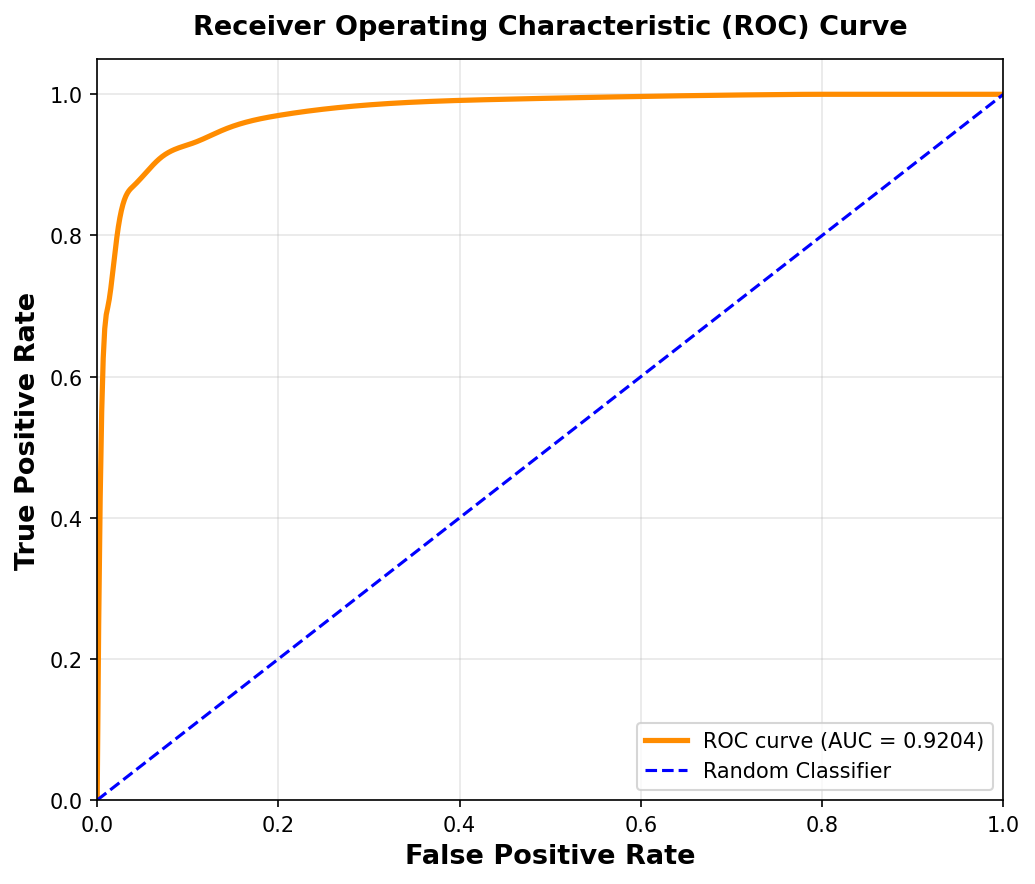
\includegraphics[width=0.85\columnwidth]{image/roc_curve.png}\\[0.3em]
{\small (a) ROC curve}\\[0.8em]
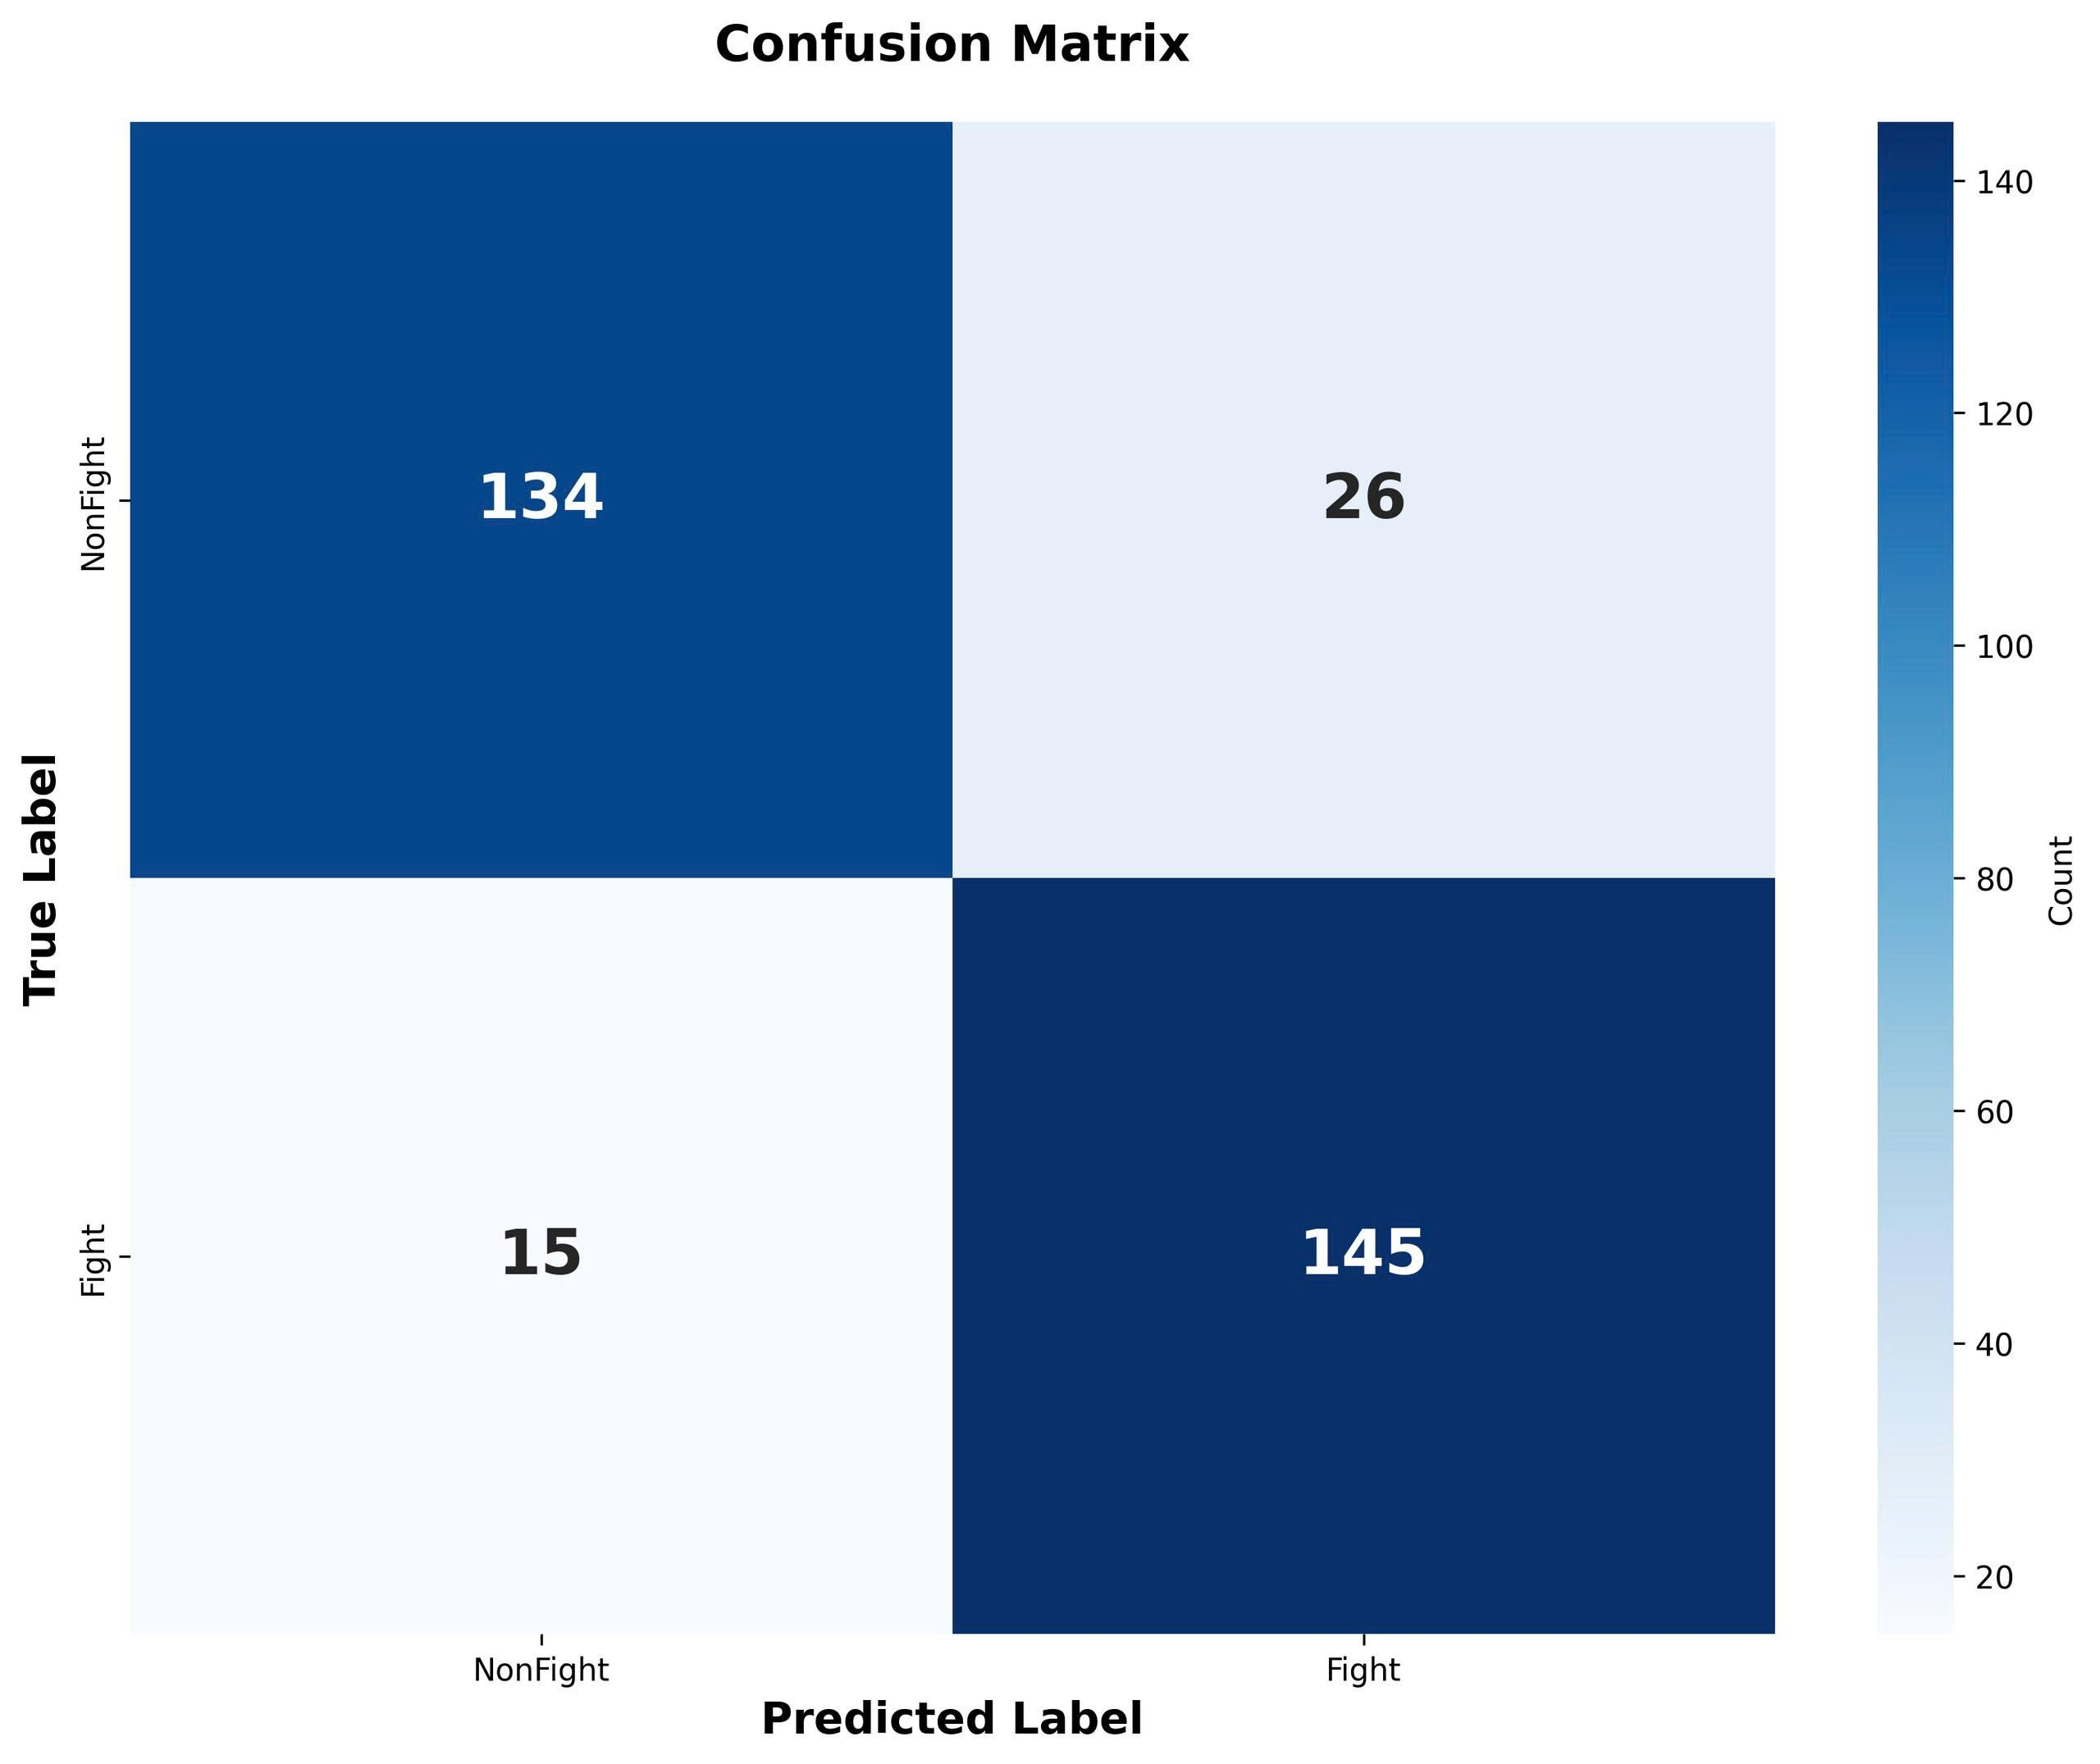
\includegraphics[width=0.85\columnwidth]{image/confusion_matrix.png}\\[0.3em]
{\small (b) Confusion matrix}
\caption{Quantitative evaluation metrics: (a) ROC curve demonstrating strong class separability, and (b) Confusion matrix detailing class-wise predictions.}
\label{fig:evaluation_metrics}
\end{figure}

The FP/FN asymmetry (61 vs.\ 40) is an intentional outcome of how we calibrate Stage~A's thresholds. In real surveillance, a missed violent event is much more costly than a spurious alert that an operator can dismiss in seconds. Stage~A is therefore tuned conservatively so that boundary-case groups get forwarded to Stage~B instead of being silently dropped.

Table~\ref{tab:latency} presents a component-wise latency breakdown measured on the RTX~2080~Ti. Stage~A components (YOLOv8, DeepSORT, optical flow, SVM) process every incoming frame in $\sim$18~ms (about 55~FPS) and run continuously. Stage~B is triggered only for the filtered candidate subset, averaging 41.72~ms per 16-frame clip. Across the test set, Stage~B activates for an average of 2.1~ROI clips per video. For a typical 30~FPS source stream lasting around 5~seconds (150 frames), the amortized Stage~B contribution is approximately $2.1 \times 41.72 / 150 \approx 0.58$~ms per CCTV frame. The effective per-frame latency is therefore Stage~A~($\sim$18~ms) plus the amortized Stage~B overhead, yielding a sustained throughput of \textbf{24~FPS} on a continuous CCTV stream.

\begin{table}[!htbp]
\centering
\footnotesize
\caption{Component-wise end-to-end latency on RTX~2080~Ti}
\label{tab:latency}
\begin{tabular}{lcc}
\hline
\textbf{Component} & \textbf{Scope} & \textbf{Latency} \\
\hline
YOLOv8 Detection            & Per frame   & 8.3~ms \\
DeepSORT Tracking           & Per frame   & 3.7~ms \\
Farneback Optical Flow      & Per frame   & 6.1~ms \\
Feature Extr. + SVM         & Per window  & $<$1~ms \\
\textbf{Stage~A Total}      & Per frame   & $\sim$18~ms \\
\hline
Swin Backbone (ROI)         & Per frame   & 2.3~ms \\
Temporal Transf. + MLP      & Per clip    & 4.8~ms \\
\textbf{Stage~B Total}      & Per clip    & \textbf{41.72~ms} \\
\hline
\textbf{End-to-end} & Per frame & \textbf{$\sim$18.6~ms / 24~FPS} \\
\hline
\end{tabular}
\end{table}


\subsection{Ablation Study}

We investigate each pipeline component through a controlled ablation, keeping the training settings fixed while varying the architecture. We evaluate four configurations: (1)~\textit{Stage~A Only}, the micro-physical SVM classifier without any deep model; (2)~\textit{Swin Only}, an ROI-based Swin Transformer performing per-frame binary classification with no temporal aggregation; (3)~\textit{Stage~B without Stage~A}, the full Swin--Temporal Transformer applied directly to all detected person-group ROIs and bypassing the kinematic filter; and (4)~\textit{Full Pipeline (A+B)}, the complete proposed framework.

\begin{table}[!htbp]
\centering
\caption{Ablation study results on the validation set (1149 clips)}
\label{tab:ablation}
\resizebox{\columnwidth}{!}{%
\begin{tabular}{|l|c|c|c|c|}
\hline
\textbf{Method} & \textbf{Acc. (\%)} & \textbf{Prec. (\%)} & \textbf{Recall (\%)} & \textbf{F1 (\%)} \\
\hline
Stage A Only (SVM) & 78.3 & 76.1 & 82.4 & 79.1 \\
Swin Only (Frame-level) & 87.19 & 84.80 & 90.62 & 87.61 \\
Stage B w/o Stage A & 89.2 & 86.5 & 91.8 & 89.1 \\
\textbf{Full Pipeline (A+B)} & \textbf{91.2} & \textbf{89.7} & \textbf{93.0} & \textbf{91.4} \\
\hline
\end{tabular}%
}
\end{table}

Stage~A alone achieves 82.4\% recall at 76.1\% precision. The gap is largely expected: momentum and directional entropy capture high-energy interactions well but cannot separate genuine violence from contact sports or aggressive play that share similar physical signatures. The SVM operates in a compact feature space with no spatial or contextual awareness, so it reaches a natural ceiling in visually complex scenes.

Adding per-frame Swin encoding without any temporal context (\textit{Swin Only}) raises accuracy to 87.19\%. Spatial features resolve many per-frame ambiguities, but clips where violence builds up gradually (through an escalation pattern that no single frame captures cleanly) stay problematic. Frame-level decisions cannot see this kind of temporal structure.

Bypassing Stage~A and running Stage~B over every detected ROI (\textit{Stage~B without Stage~A}) yields 89.2\% accuracy. This setting pushes about $5.8\times$ more candidate ROIs through the deep model per video relative to the filtered pipeline. We get this ratio by comparing the mean active-ROI count per test clip with and without Stage~A. The inflated candidate set raises GPU load and exposes the recognizer to more background clutter, which in turn pushes the false-positive rate above that of the filtered variant.

The complete two-stage pipeline reaches 91.2\% accuracy and a 91.4\% F1-score, a 2.3 percentage-point gain in F1 over Stage~B alone. Stage~A improves input quality by removing most non-violent candidates before deep inference runs, while Stage~B handles the ambiguous cases that kinematic features cannot resolve on their own. Neither module reproduces this performance independently, and the gain is achieved without a proportional increase in computational cost because Stage~B only fires on the reduced filtered set.

\subsection{Hyperparameter Sensitivity Analysis}

To check that the system is not over-tuned to specific hyperparameter values, we ran sensitivity sweeps over the three knobs that matter most: the adaptive grouping scale factor $K$, the sliding window size $N$, and the temporal clip length $T$. We held everything else at its default while sweeping one parameter at a time.

\begin{table}[!htbp]
\centering
\caption{Hyperparameter sensitivity on the validation set (1149 clips)}
\label{tab:sensitivity}
\begin{tabular}{|l|c|c|c|}
\hline
\textbf{Parameter} & \textbf{Value} & \textbf{Acc. (\%)} & \textbf{F1 (\%)} \\
\hline
\multirow{3}{*}{$K$ (grouping scale)} & 1.00 & 88.4 & 87.6 \\
 & \textbf{1.50 (default)} & \textbf{91.2} & \textbf{91.4} \\
 & 2.00 & 90.1 & 89.7 \\
\hline
\multirow{3}{*}{$N$ (window size)} & 5  & 89.3 & 88.9 \\
 & \textbf{10 (default)} & \textbf{91.2} & \textbf{91.4} \\
 & 20 & 91.1 & 90.8 \\
\hline
\multirow{3}{*}{$T$ (clip length)} & 8  & 89.7 & 89.2 \\
 & \textbf{16 (default)} & \textbf{91.2} & \textbf{91.4} \\
 & 32 & 91.5 & 91.0 \\
\hline
\end{tabular}
\end{table}

As shown in Table~\ref{tab:sensitivity}, the system achieves peak performance at the default settings and degrades gracefully outside these values. For $K$: a smaller value (1.00) under-groups individuals in crowded scenes, reducing Stage~B candidate coverage and dropping F1 by 3.8 points; a larger value (2.00) over-groups unrelated bystanders, increasing false positives and reducing F1 by 1.7 points. For $N$: a window of 5~frames captures insufficient kinematic evidence for reliable SVM pre-filtering, while 20~frames introduces temporal lag without proportional accuracy gain. For $T$: increasing clip length to 32~frames yields only a 0.4-point F1 improvement at double the Stage~B computational cost, confirming $T=16$ as the optimal efficiency--accuracy trade-off.

\subsection{Performance on Unified In-the-Wild Dataset}

\begin{table}[!htbp] 
\centering
\caption{Comparison with state-of-the-art methods on the Unified Benchmark}
\label{tab:sota}
\resizebox{\linewidth}{!}{%
\begin{tabular}{|l|c|c|c|c|} 
\hline
\textbf{Method} & \textbf{Acc. (\%)} & \textbf{F1 (\%)} & \textbf{AUC (\%)} & \textbf{FPS} \\
\hline
CNN-LSTM \cite{patel_realtime_2021} & 82.4 & 81.7 & 88.1 & 18.5 \\
C3D \cite{ding_violence_2014} & 85.3 & 84.9 & 90.2 & 22.1 \\
CNN+RNN \cite{traore_violence_2024} & 86.5 & 85.8 & 91.1 & 19.8 \\
X3D \cite{pathak_streamlining_2024} & 87.2 & 86.4 & 91.5 & 28.3 \\
Attention-based \cite{pan_violence_2022} & 87.9 & 87.1 & 91.8 & 20.4 \\
\textbf{Proposed (A+B)} & \textbf{91.2} & \textbf{91.4} & \textbf{92.04} & 24.0 \\
\hline
\end{tabular}%
}
\end{table} 

Cross-paper comparisons in violence detection are hard to interpret fairly. Different methods evaluate on different splits, on proprietary datasets, or on hardware configurations that vary considerably. To sidestep these confounds, we re-implemented five representative baselines (C3D~\cite{ding_violence_2014}, CNN-LSTM~\cite{patel_realtime_2021}, CNN+RNN~\cite{traore_violence_2024}, X3D~\cite{pathak_streamlining_2024}, and the attention-based network~\cite{pan_violence_2022}) from their original descriptions and trained each one on the Unified Benchmark under matched conditions. All baselines were optimized with AdamW (initial lr~$= 1\times10^{-4}$, weight decay~$= 0.01$), cosine annealing over 50 epochs, batch size of 8, and the same 80/20 stratified split. For C3D and X3D, publicly available ImageNet-pretrained weights were used as initialization; CNN-LSTM, CNN+RNN, and the attention-based model were initialized from random weights following specifications in their source papers. All models receive the same 16-frame ROI clips at $224\times224$ resolution as input. Table~\ref{tab:sota} summarizes accuracy, F1, AUC, and per-clip inference speed for all methods.

Our framework achieves the highest accuracy (91.2\%) and F1-score (91.4\%) in this comparison. Among the baselines, C3D and X3D reach 85.3\% and 87.2\% respectively. A non-trivial share of their errors comes from hard-negative test sequences such as aggressive dancing, contact sports, and dense crowd dynamics, where the global spatio-temporal statistics across the full frame can look like violence. Neither architecture has a mechanism for isolating the person-group interaction region, so background motion and bystander movements get folded into the feature representation and push the false-positive rate up.

CNN-LSTM~\cite{patel_realtime_2021} scores 82.4\% accuracy. Recurrent temporal encoding over dense spatial features is vulnerable to partial occlusions within a clip: a missed or noisy detection over just a few frames can corrupt the hidden state and degrade classification for the remainder of the sequence. The attention-based network~\cite{pan_violence_2022} mitigates some of this by selectively weighting regions, reaching 87.9\%, but it still operates on full frames and must allocate capacity to bystanders and static background.

The structural advantage of our pipeline is that Stage~A gates the input spatially before any deep inference is triggered. ROIs reaching Stage~B have already passed a kinematic sanity check, so the input is cleaner and more focused. This gating reduces the feature-level confusion that full-frame models hit and accounts for most of the performance gap visible in Table~\ref{tab:sota}.

The framework achieves 93.0\% recall with precision held at 89.7\%. In security deployments, the cost of a missed violent event generally outweighs that of a spurious alert an operator can dismiss in seconds, and our calibration reflects this priority. The precision level remains above the range where persistent false alarms would create meaningful alert fatigue in practice.

In terms of throughput, Stage~B averages 41.72~ms per 16-frame clip on the RTX~2080~Ti. Combined with Stage~A's $\sim$18~ms per frame and the fact that Stage~B only fires on a small candidate subset, the end-to-end pipeline sustains roughly 24~FPS on a continuous feed, which is competitive with the baselines we tested and sufficient for real-time deployment. Because Stage~B is bypassed entirely for candidates rejected by Stage~A, actual system throughput is higher than the isolated Stage~B per-clip figure suggests.


\section{Conclusion}

We presented a two-stage violence detection pipeline that we built around one main idea: the deep model should not see frames it does not need to see. Stage~A is a cheap kinematic filter (adaptive proximity grouping, 7-dimensional motion descriptor, RBF-SVM gatekeeper) that drops about two thirds of the candidate windows before any GPU work begins. Stage~B is a Swin Transformer spatial encoder followed by a small Temporal Transformer, applied only to the surviving ROI clips. On a unified benchmark of 1,149 held-out clips taken from six public datasets and our own PTIT footage, the full system reaches 91.2\% accuracy, 91.4\% F1, and 92.04\% AUC-ROC at roughly 24~FPS on a single RTX~2080~Ti.

\vspace{0.15cm}
\noindent\textbf{Limitations.} The framework still has several blind spots that we want to flag for anyone considering deployment.

The kinematic filter assumes that violence happens between at least two tracked persons. That assumption breaks in two situations we have hit ourselves. One is total occlusion, where the bounding boxes of the people fighting collapse into a single blob and the centroid we use for grouping becomes unreliable. The other is single-person violence (self-harm or weapon attacks aimed at someone off-camera), where there is no interaction pair for Stage~A to form, so no candidate ever reaches Stage~B.

The SVM gatekeeper is set to favor recall, so it lets through more borderline cases than a balanced classifier would. Even so, slow-escalation attacks can slip past it: if the aggressor moves deliberately and peak acceleration never crosses our 15-pixel-per-height threshold inside any 10-frame window, the clip is rejected at the gate and Stage~B never sees it. We have observed this most clearly in restraint footage and in pre-fight argument sequences. Any sample dropped here is gone for good.

Finally, the entire pipeline depends on YOLOv8 producing usable tracks. Low-light footage, heavy rain, fisheye distortion at the edges of the frame, and extreme scale changes between near and far subjects all reduce the number of tracks available for grouping. When tracks disappear, real fights are silently filtered out before any feature is computed. Detector ensembling or fine-tuning on a per-camera profile would help, and we treat that as a prerequisite for any production rollout rather than a research nice-to-have.

\vspace{0.15cm}
\noindent\textbf{Future Work.} On the modeling side, we plan to swap the spatial encoder for Swin Transformer~V2~\cite{liu_swin_2022} or one of the mobile-friendly variants, since the current Swin~Tiny backbone is the dominant cost on edge hardware. We are also experimenting with a cross-modal extension that fuses synchronized audio, because some visually ambiguous cases (sports cheering, animated greetings) are trivially separable once a microphone is added.

On the task side, the binary classifier is informative but coarse. Operators we have spoken to want more granularity, particularly the distinction between assault, robbery, weapon display, and crowd stampede, and ideally a severity score so that low-stakes alerts can be deferred. We are working on a multi-class extension with a small severity regression head.

On the deployment side, we want to reduce the YOLOv8 dependency by trying keypoint-based proximity estimation, which should be more robust to partial occlusion than bounding-box centroids. We also intend to run longer pilots in live settings (campus and transit) to collect failure cases that no curated benchmark currently exposes, and to audit demographic bias before any such system is allowed to flag people in real time.

\bibliographystyle{ieeetr}
\bibliography{ViolanceDetect}

\end{document}
